\documentclass[11pt]{homework}

\usepackage[UTF8]{ctex}
\usepackage{graphicx}
\usepackage{float} 
\usepackage{subfigure}
\usepackage{color}
\usepackage{listings}
\usepackage{url}
\lstset{
  showspaces=false,
  showtabs=false,
  breaklines=true,
  showstringspaces=false,
  breakatwhitespace=true,
  commentstyle=\color{green},
  keywordstyle=\color{blue},
  stringstyle=\color{red},
  basicstyle=\ttfamily,
  moredelim=[il][\textcolor{pgrey}]{$$},
  moredelim=[is][\textcolor{pgrey}]{\%\%}{\%\%}
}

\newcommand{\hwname}{封钰震}
\newcommand{\hwemail}{1951362}
\newcommand{\hwtype}{作业}
\newcommand{\hwnum}{5-Java Web}
\newcommand{\hwclass}{Java语言程序设计}
\newcommand{\hwlecture}{}
\newcommand{\hwsection}{}

\usepackage{lipsum}

\begin{document}
\maketitle

\section*{写在前面}

本次作业可通过\verb|47.103.73.100:8080/eRestaurant|进行访问,其中:
\begin{itemize}
  \item 后台登录请点击\url{http://47.103.73.100:8080/eRestaurant/admin/toLogin},用户名为\verb|Admin|,密码为\verb|123456|;
  \item 用户点餐请点击\url{http://47.103.73.100:8080/eRestaurant/user/toLogin};
\end{itemize}

\section*{编程环境}

  \subsection*{硬件环境}
  \begin{itemize}
    \item 型号名称:MacBook Pro
    \item 处理器名称:Dual-Core Intel Core i5
    \item 内存:8 GB
  \end{itemize}

  \subsection*{软件环境}
  \begin{itemize}
    \item 操作系统:macOS 10.15.7(本地)
  \end{itemize}

  \subsection*{运行环境}
  \begin{itemize}
    \item JDK 14.0.2(本地)
    \item OpenJDK 11.0.12(云服务器)
    \item MySQL 5.7.34(云服务器)
    \item Tomcat 8.5.41(云服务器)
  \end{itemize}

\section*{设计思想}

  \subsection*{系统设计}
  本系统使用Spring Boot+Thymeleaf+MyBatis实现各个模块,Web服务器使用Tomcat,数据库采用的是MySQL,集成开发环境为IDEA Edu。该平台分为两个子系统,一是后台管理子系统,一是前台点单子系统。两个子系统的功能需求与模块划分如图\ref{系统设计}所示。

  \begin{figure}[htb]
    \centering
    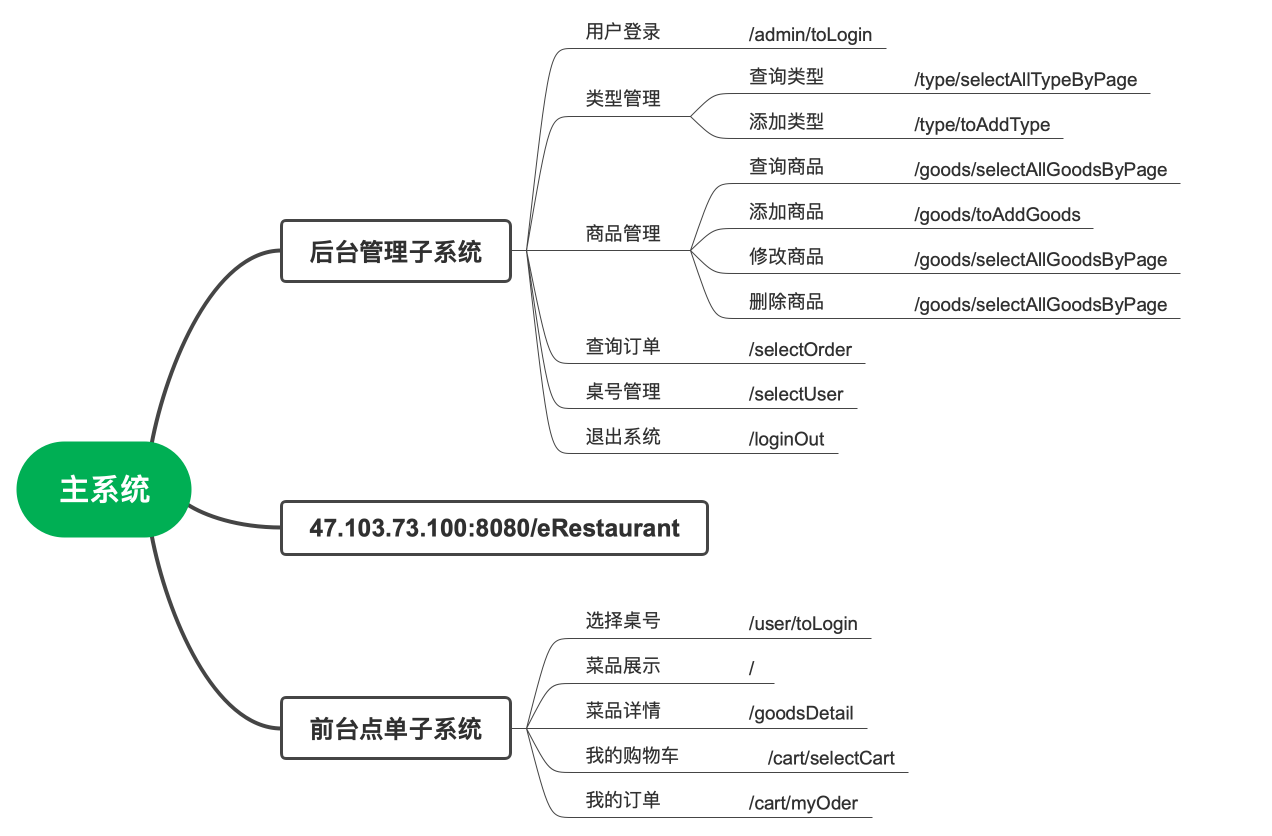
\includegraphics[width=0.9\textwidth]{系统设计}
    \caption{系统设计}
    \label{系统设计}
  \end{figure}

  \subsection*{数据库设计}
  本系统采用加载纯Java数据库驱动程序的方式连接MySQL 5.7数据库。在MySQL 5.7中创建数据库\verb|restaurant_web|,并在其中创建6张与系统相关的数据表:管理员、用户、商品类型、商品、订单、订单详情。数据库设计的ER图如图\ref{ER图}所示。

  \begin{figure}[htb]
    \centering
    \includegraphics[width=0.8\textwidth]{ER图}
    \caption{ER图}
    \label{ER图}
  \end{figure} 

\section*{执行过程}

  \subsection*{部署(即“说明书”)}

  通过\verb|Maven|打包项目成\verb|jar|包,如图\ref{打包}所示。
  \begin{figure}[htb]
    \centering
    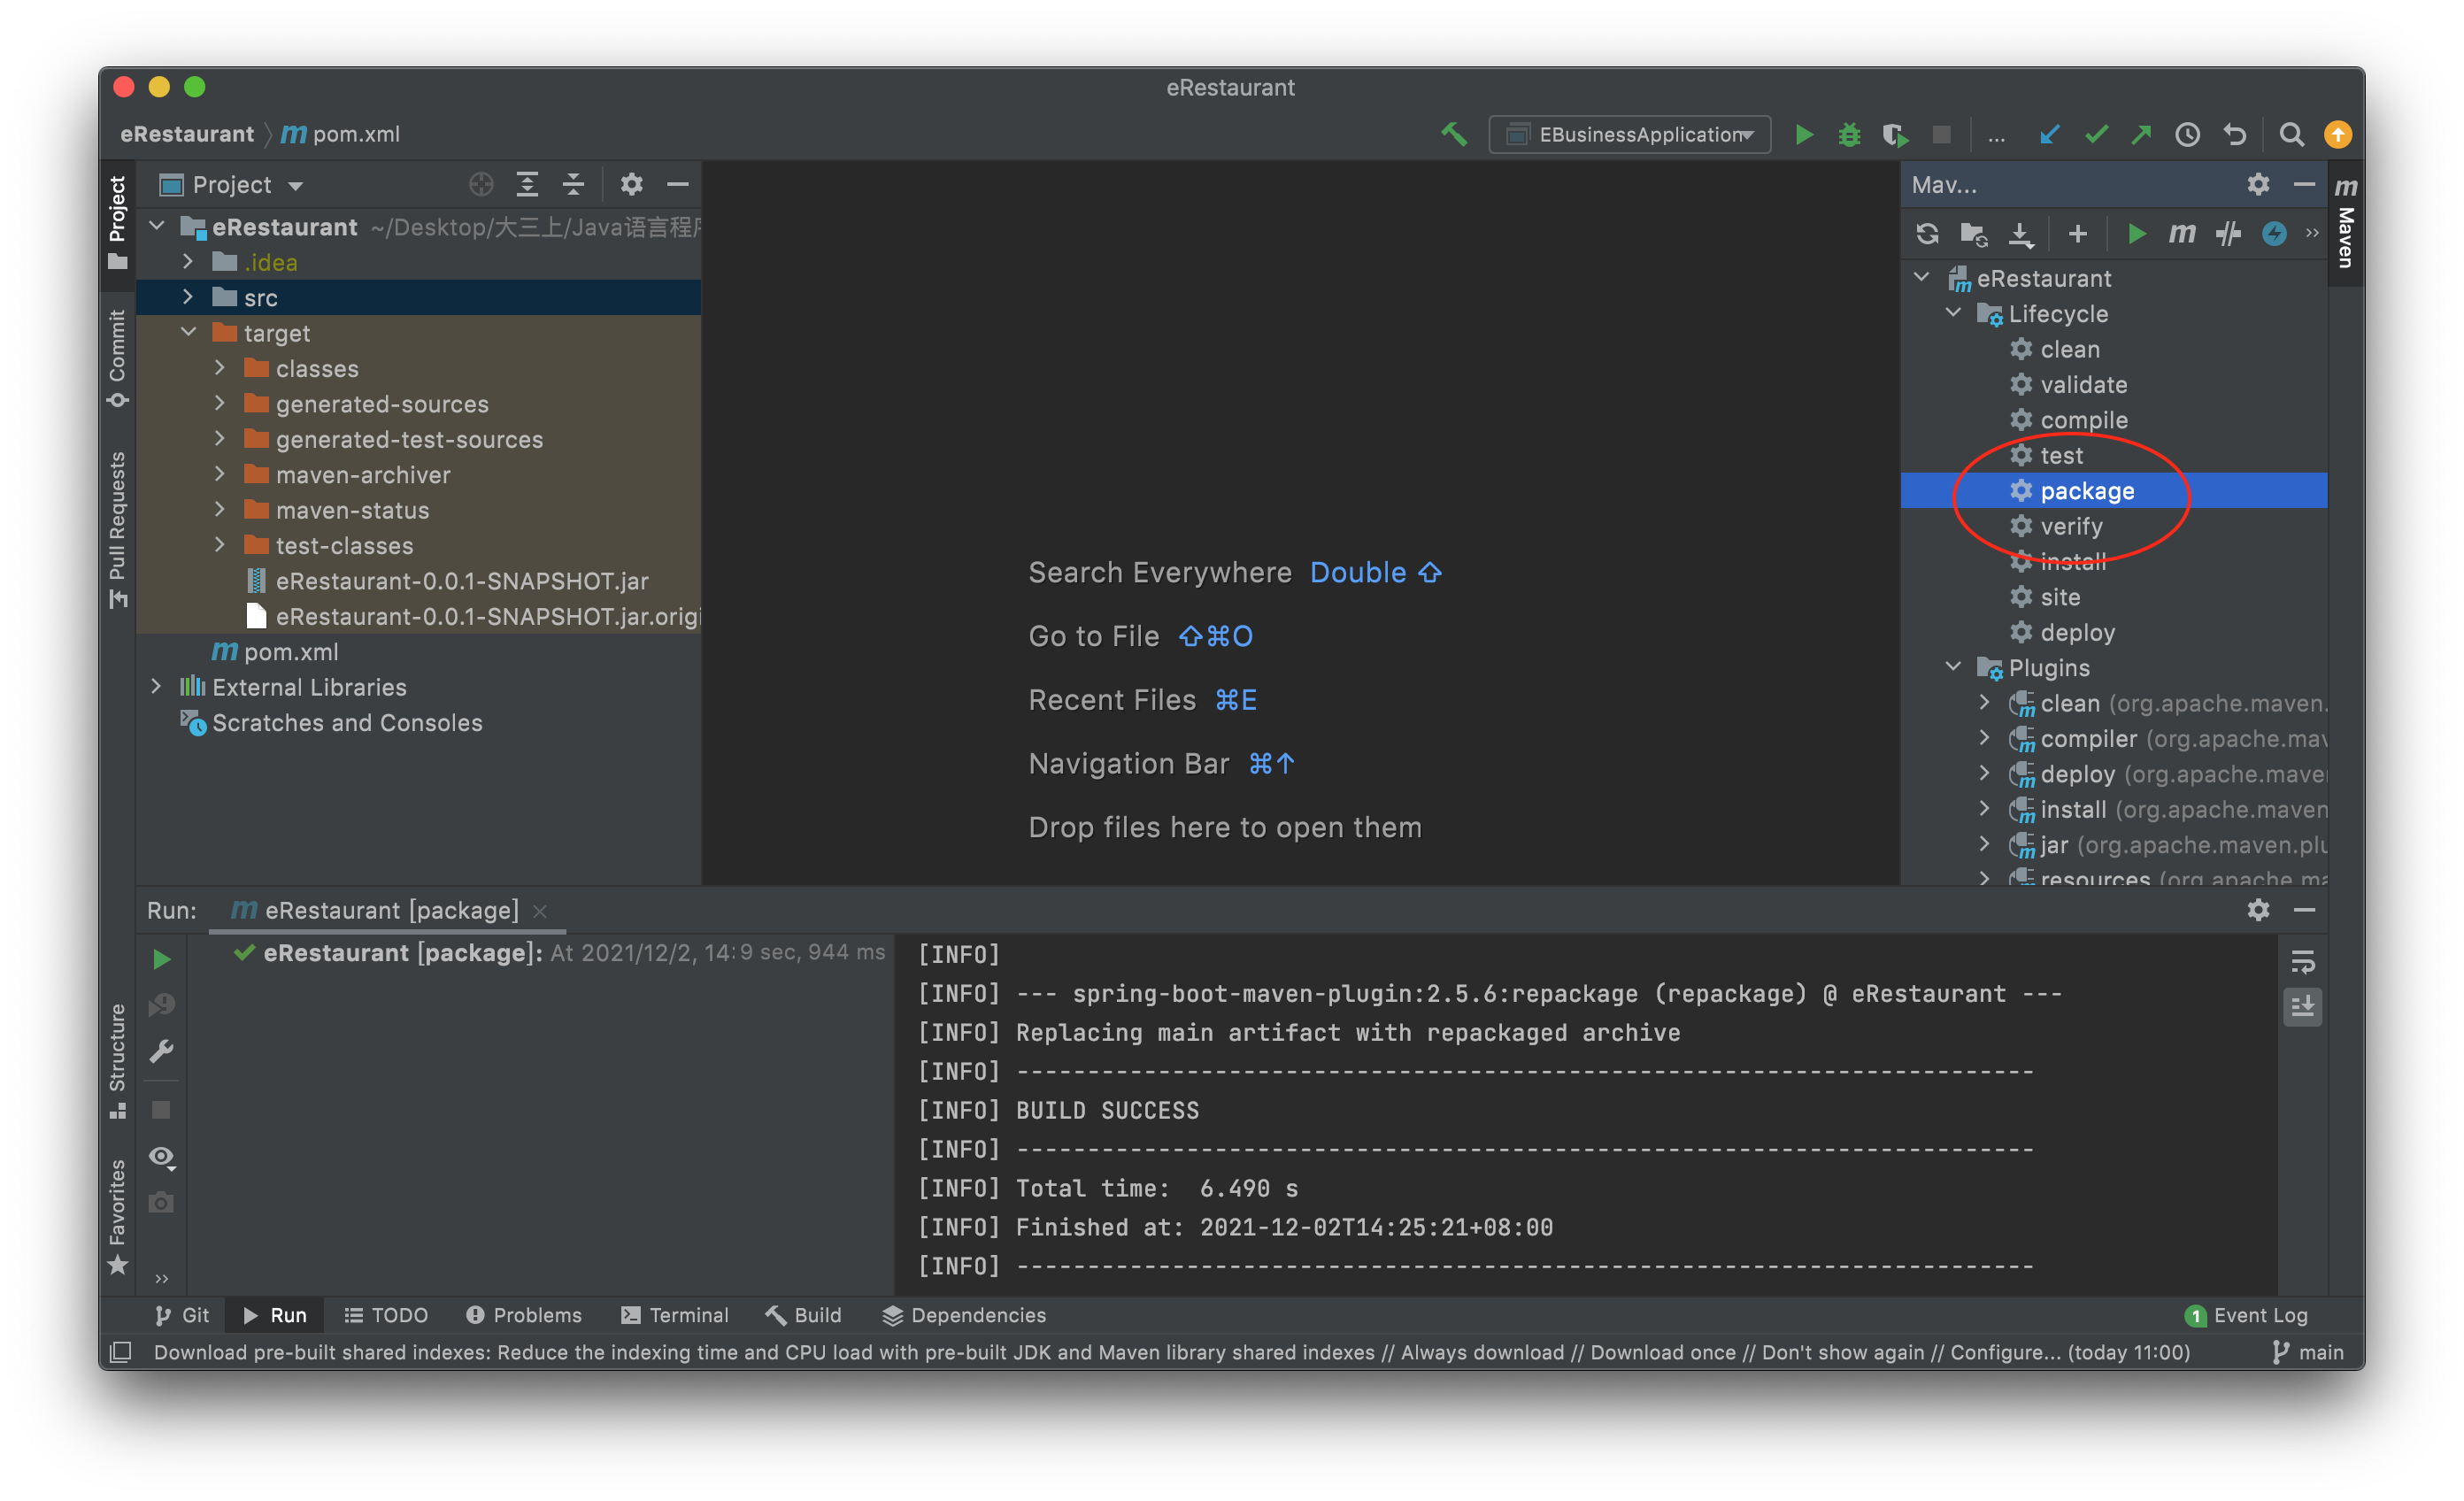
\includegraphics[width=0.8\textwidth]{打包}
    \caption{打包}
    \label{打包}
  \end{figure}

  
  然后通过\verb|scp|将\verb|jar|包上传至云服务器上Tomcat对应的文件夹中,如图\ref{上传}所示。
  \begin{figure}[htb]
    \centering
    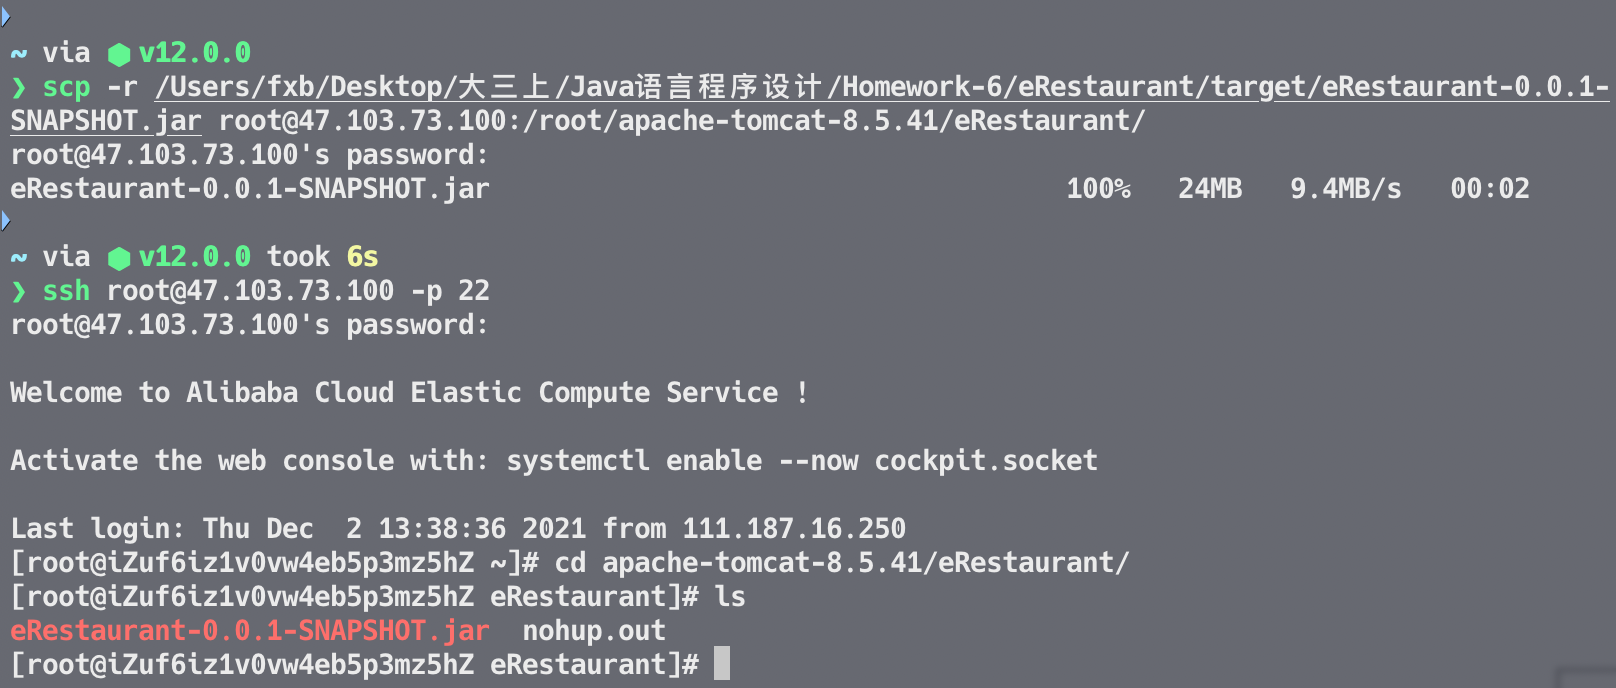
\includegraphics[width=\textwidth]{上传}
    \caption{上传}
    \label{上传}
  \end{figure}
  
  再通过\verb|java -jar|命令并使用\verb|nohup|不挂断地运行命令,如图\ref{部署}所示。
  \begin{figure}[htb]
    \centering
    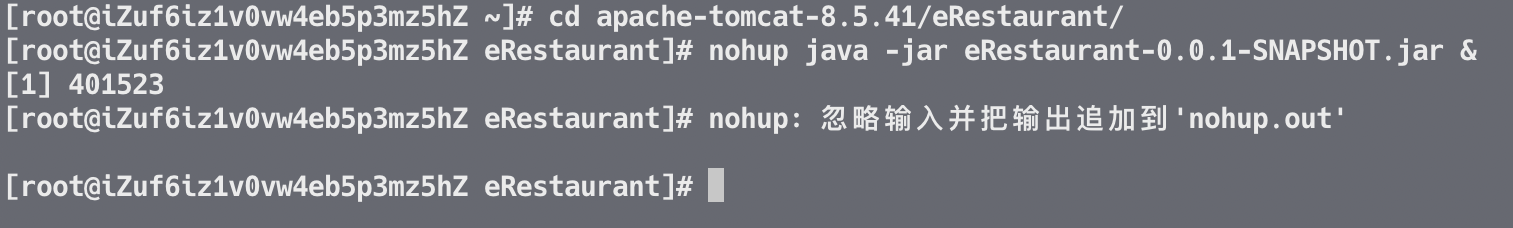
\includegraphics[width=\textwidth]{部署}
    \caption{部署}
    \label{部署}
  \end{figure}

  打开文件\verb|nohup.out|查看输出,可以看到部署成功,如图\ref{部署成功}所示。
  \begin{figure}[htb]
    \centering
    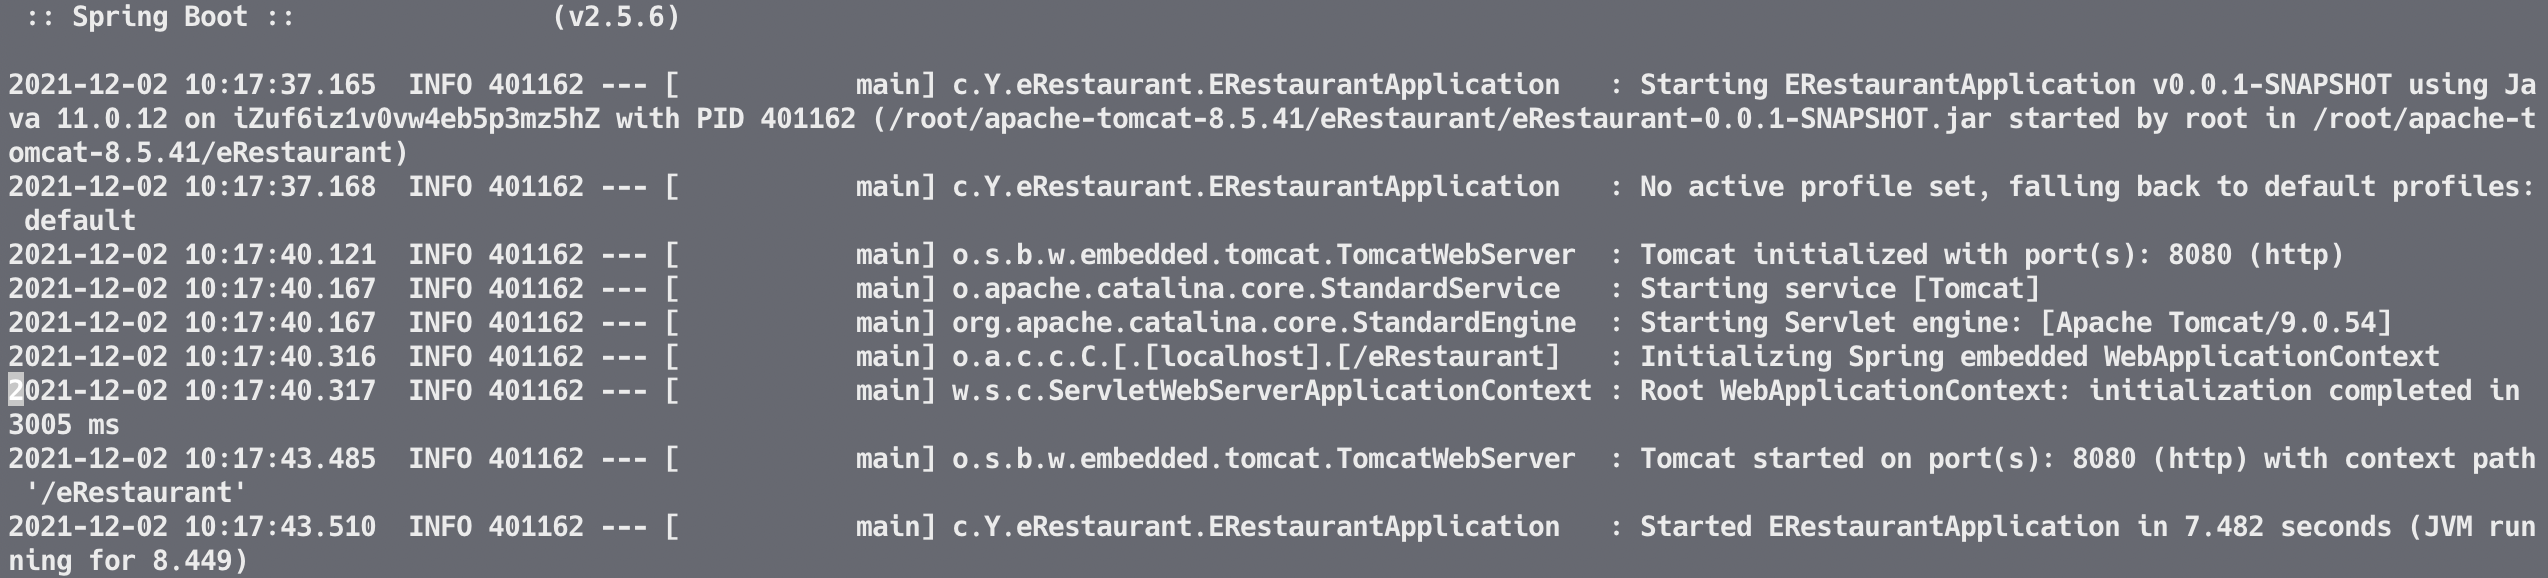
\includegraphics[width=\textwidth]{部署成功}
    \caption{部署成功}
    \label{部署成功}
  \end{figure}

  以下将展示本系统的主要界面。

  \subsection*{前台}

  如图\ref{用户选择桌号}-\ref{我的订单}所示。

    \begin{figure}[h]
      \centering
      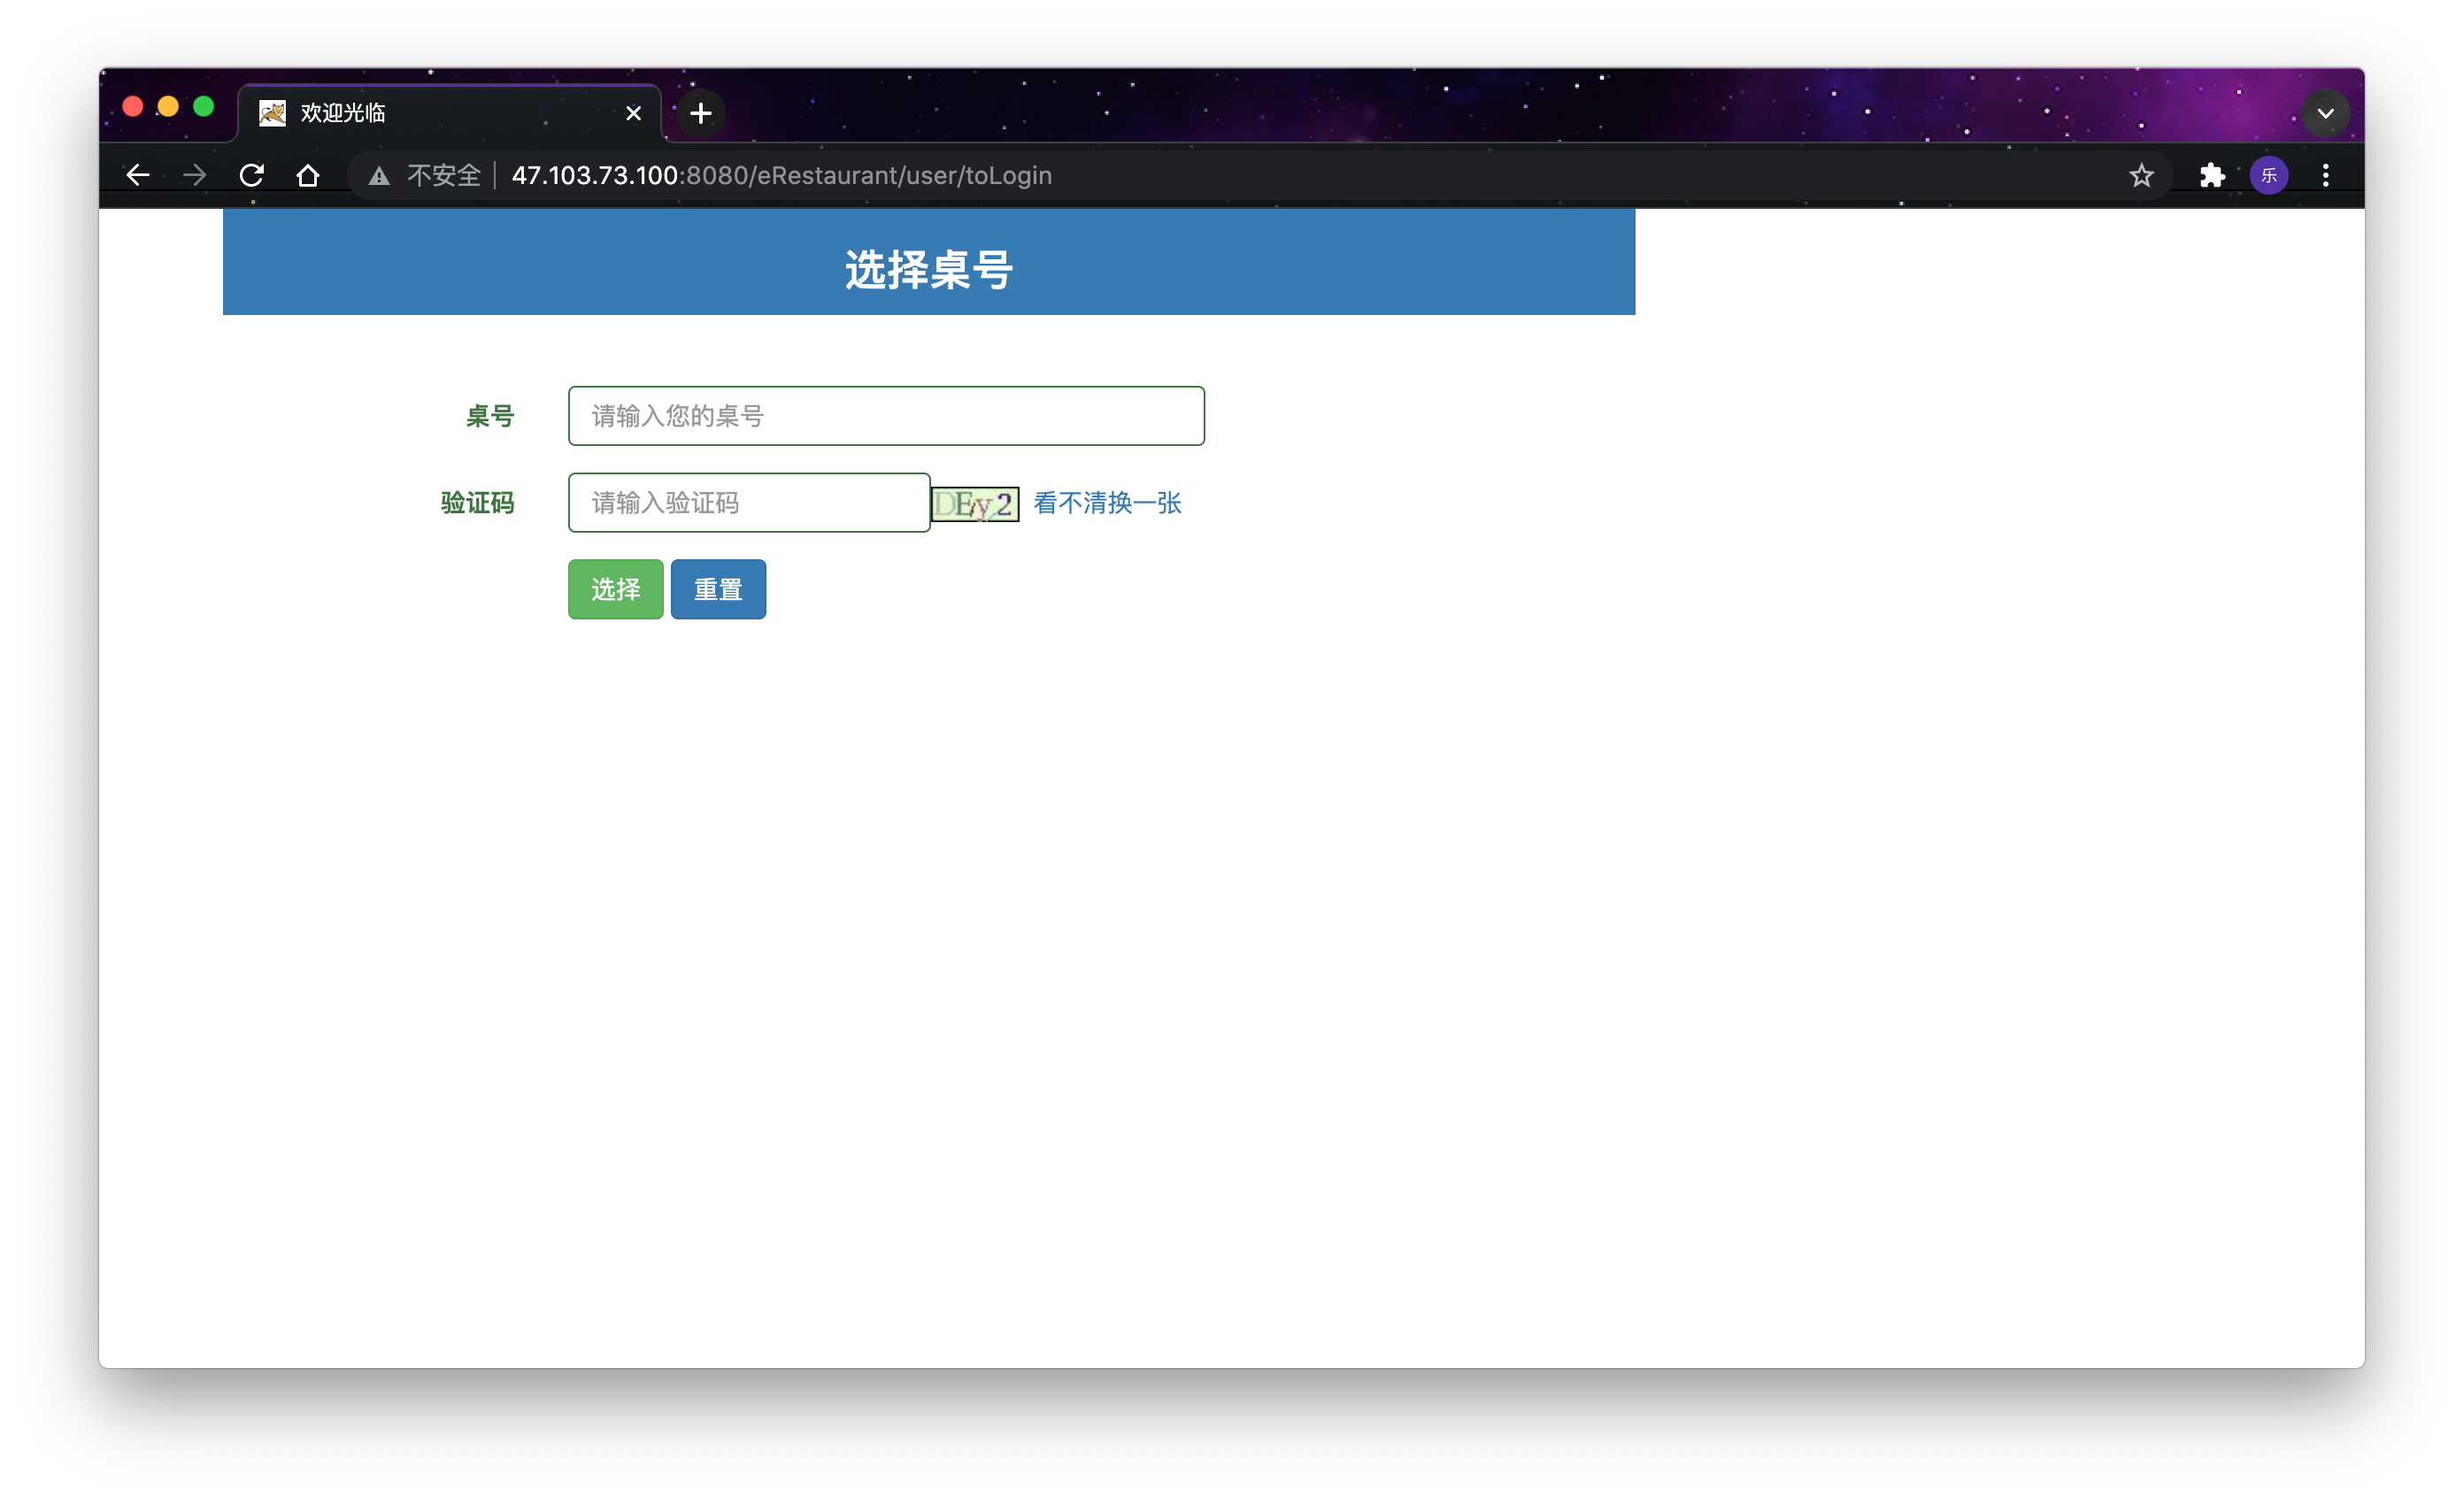
\includegraphics[width=0.8\textwidth]{用户选择桌号}
      \caption{用户选择桌号}
      \label{用户选择桌号}
    \end{figure}

    \begin{figure}[h]
      \centering
      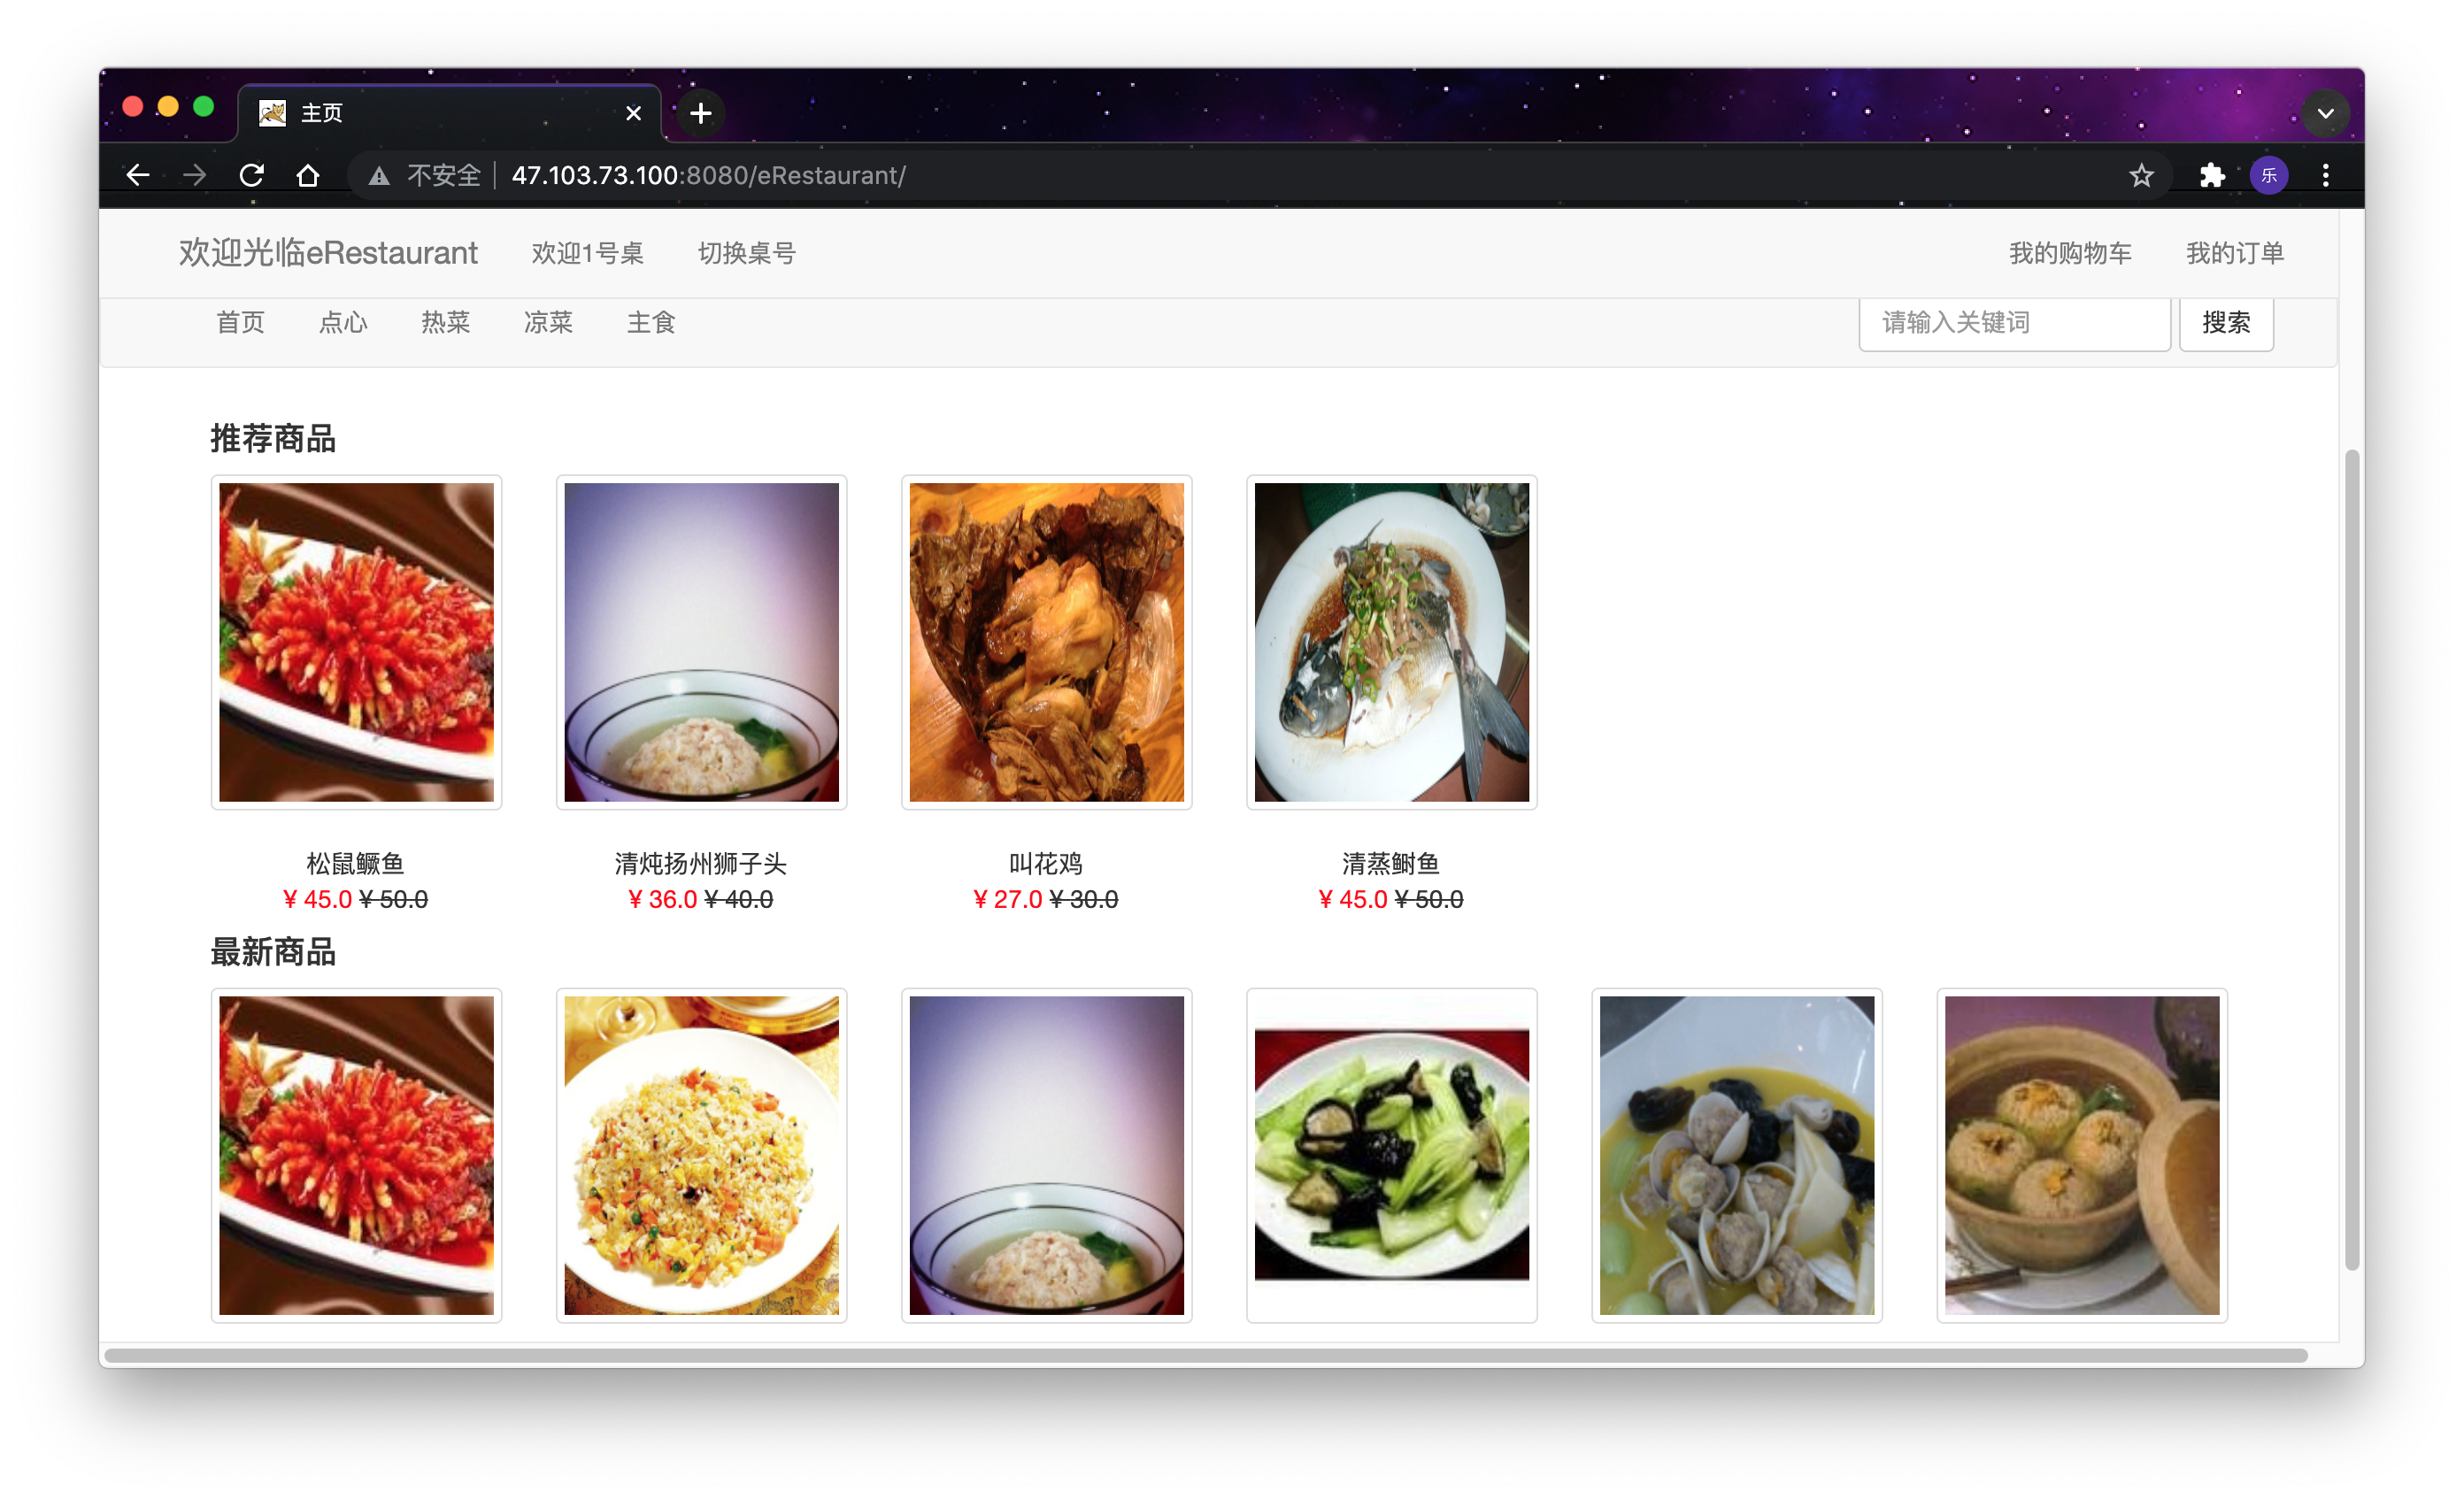
\includegraphics[width=0.8\textwidth]{菜品总览}
      \caption{菜品总览}
      \label{菜品总览}
    \end{figure}

    \begin{figure}[h]
      \centering
      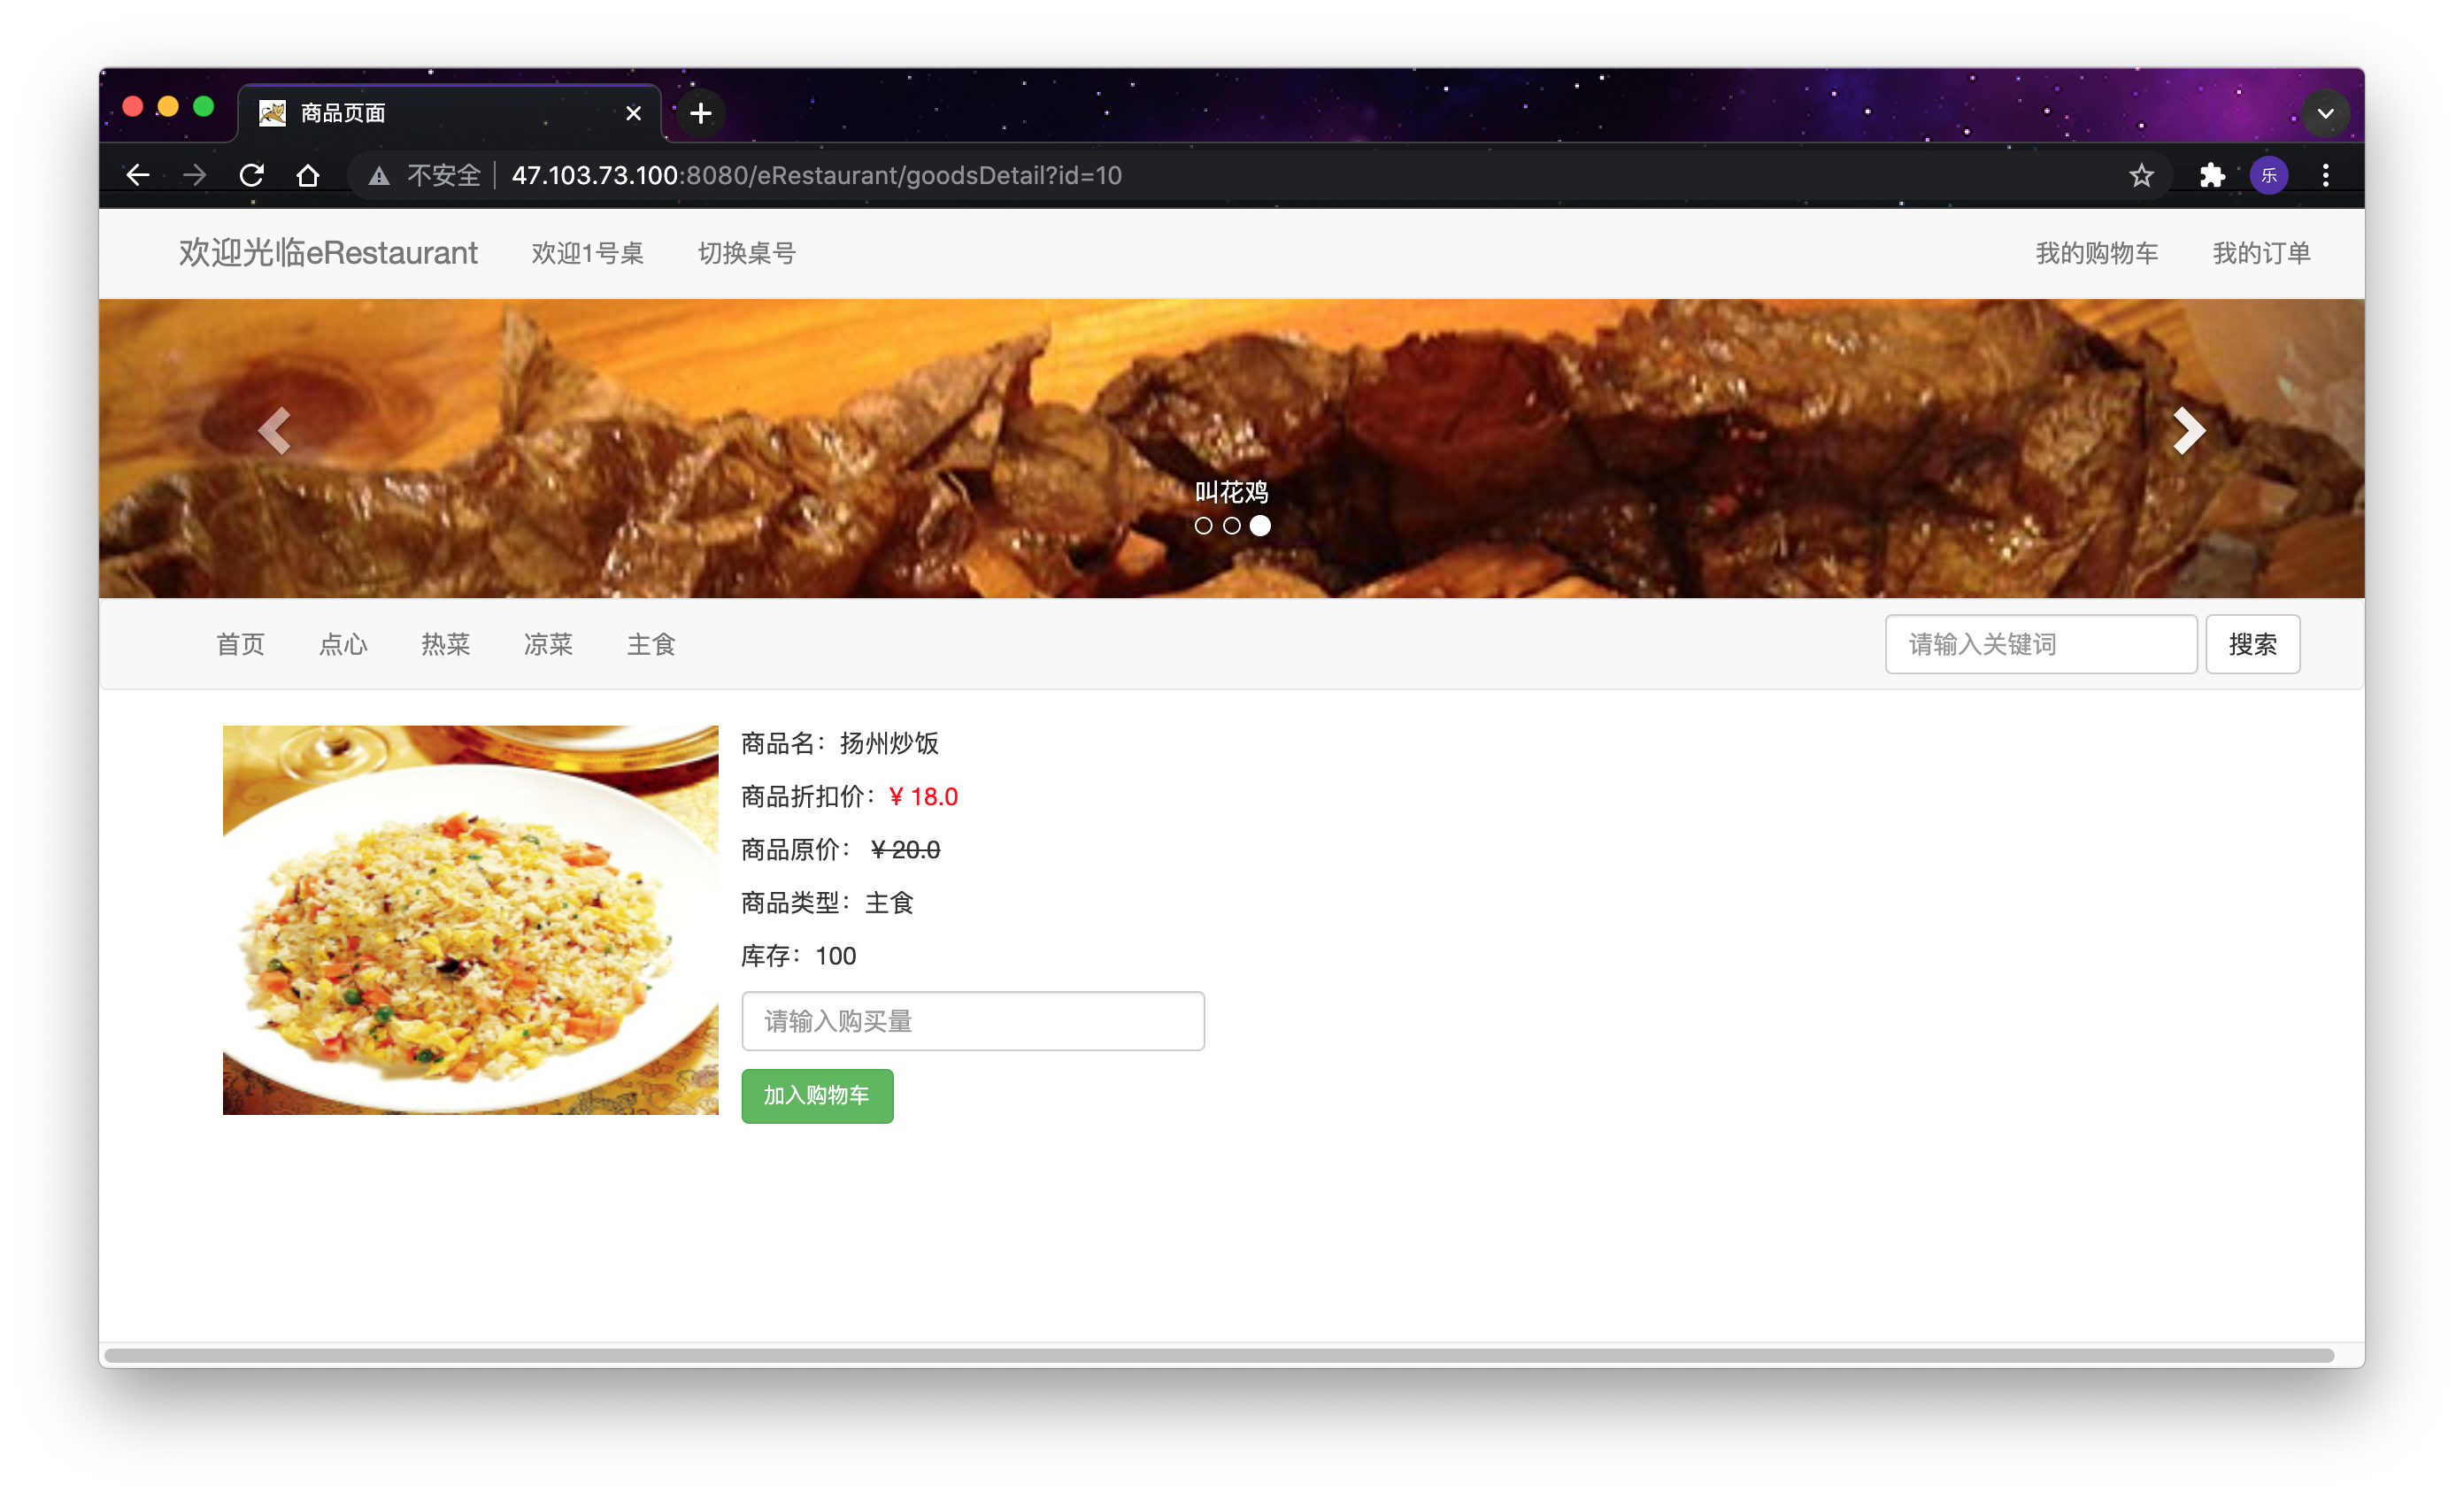
\includegraphics[width=0.8\textwidth]{菜品详情}
      \caption{菜品详情}
      \label{菜品详情}
    \end{figure}

    \begin{figure}[h]
      \centering
      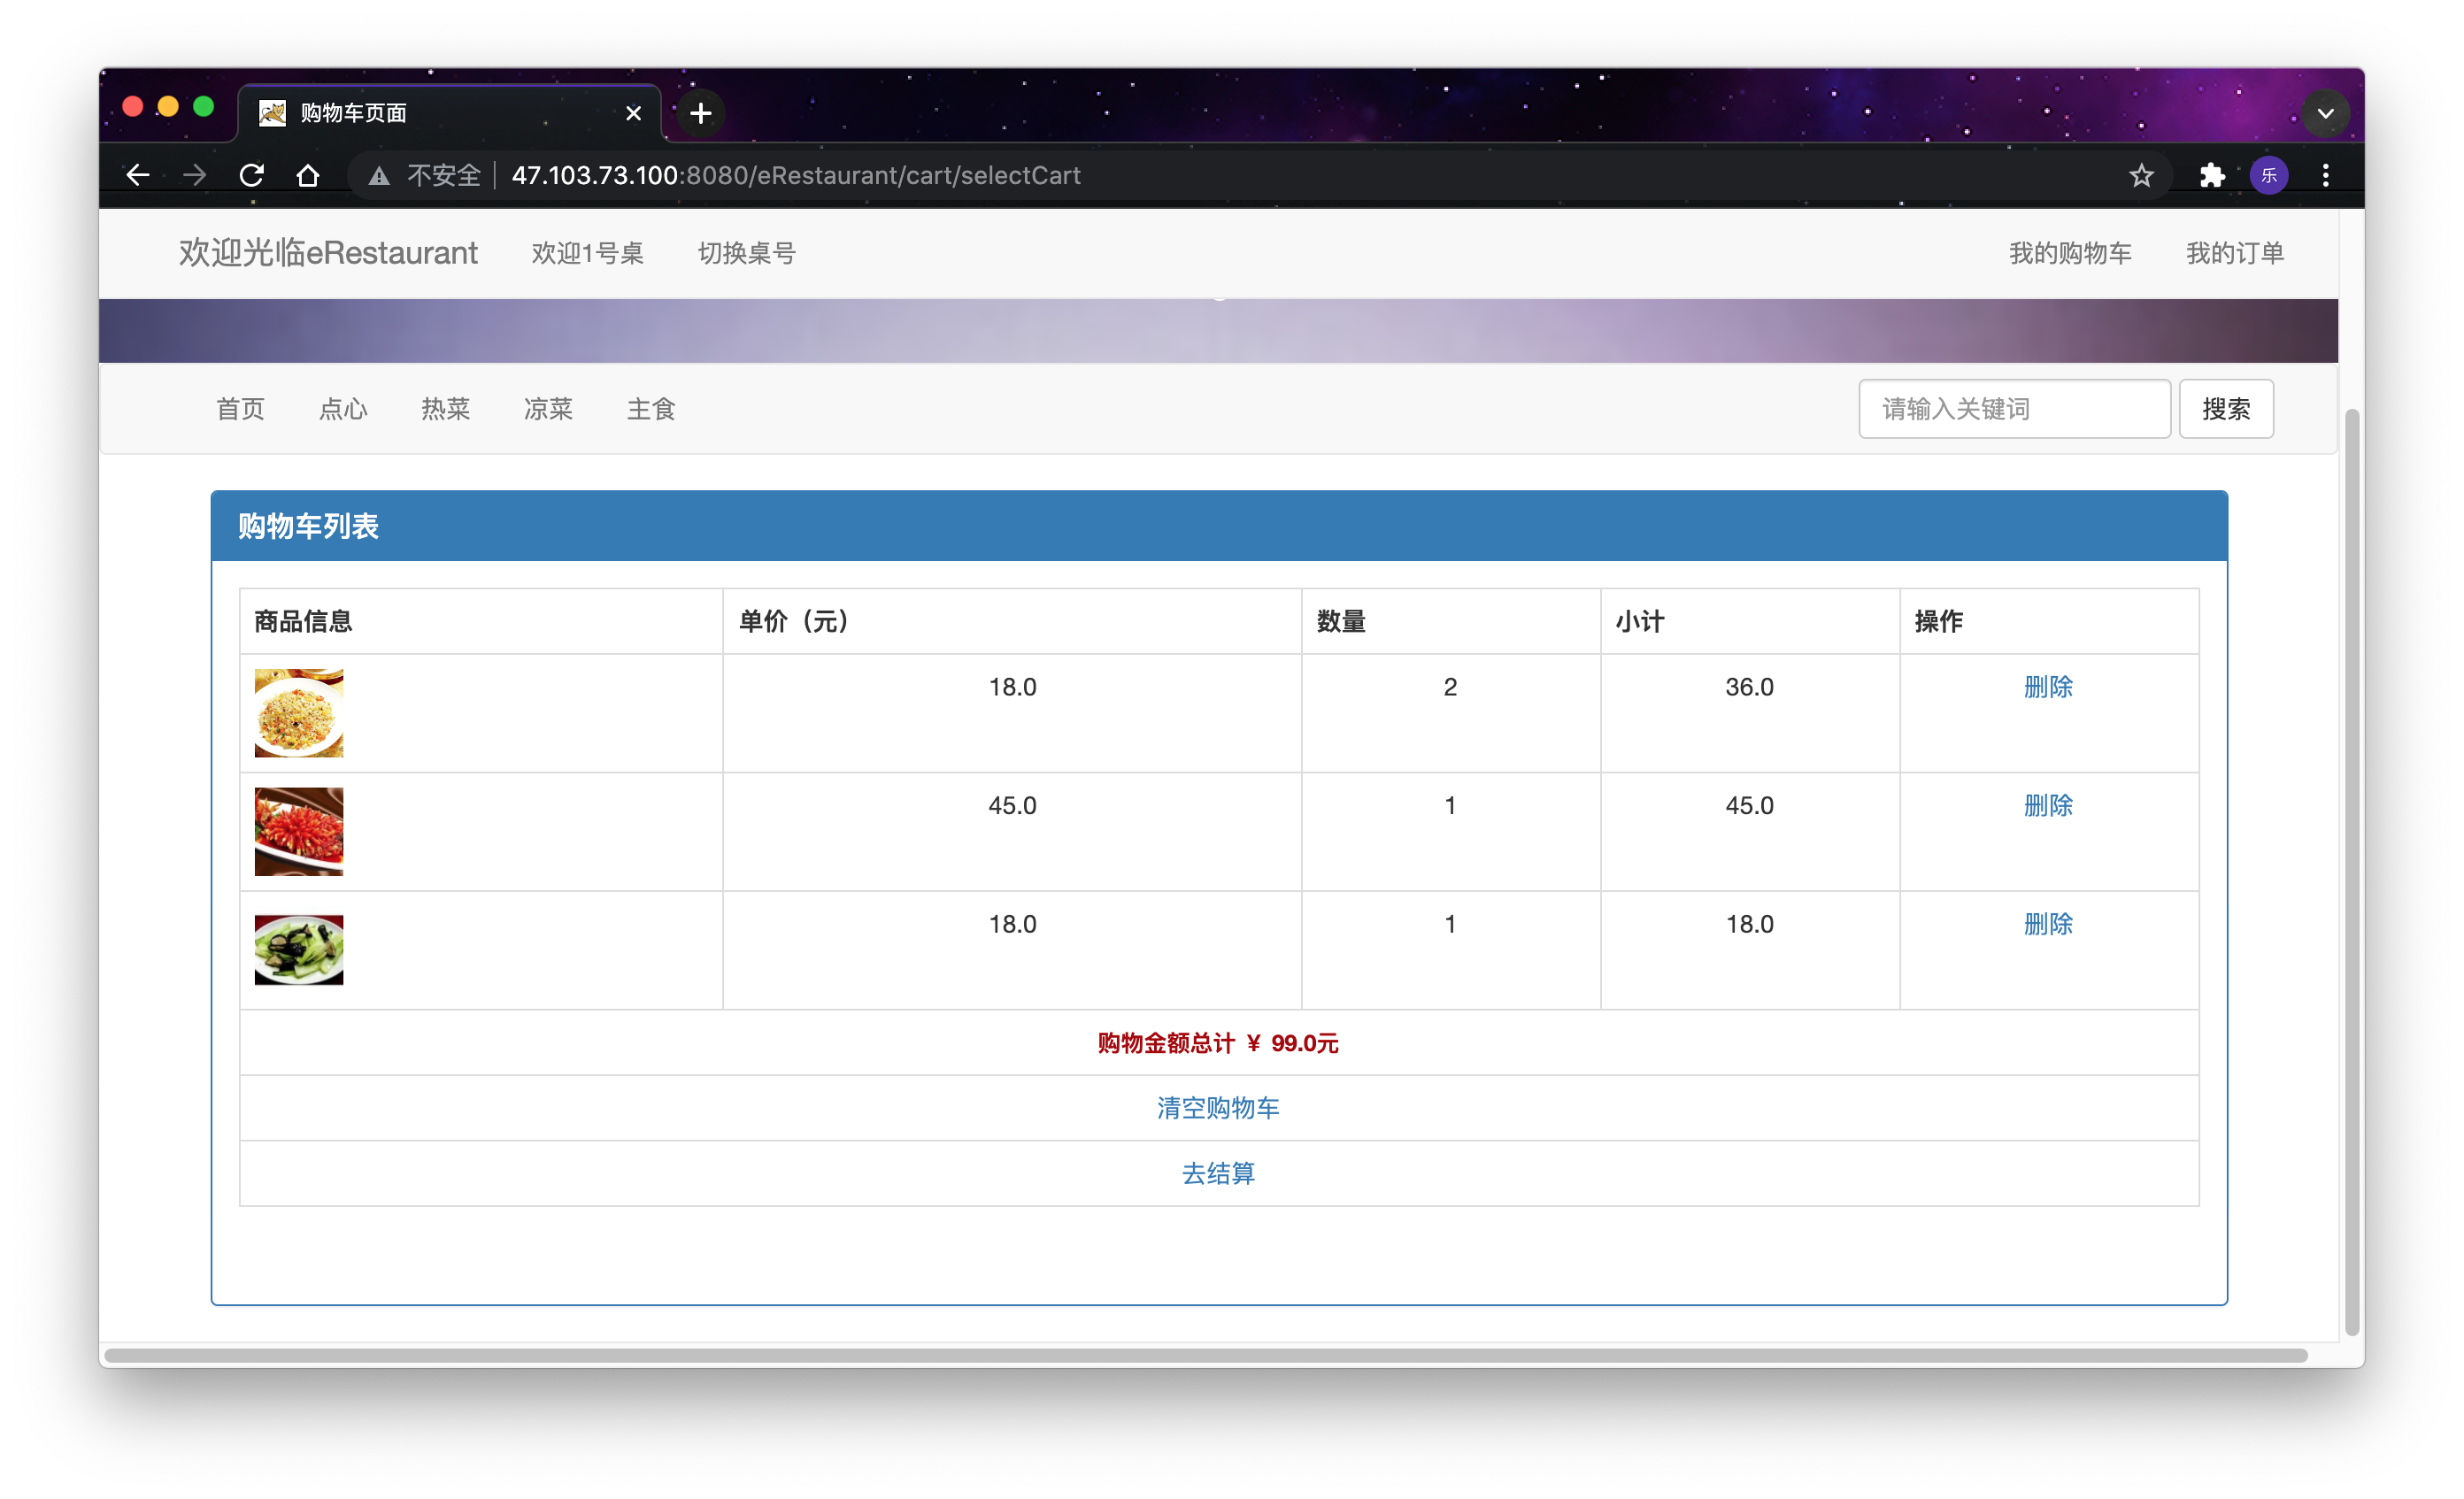
\includegraphics[width=0.8\textwidth]{我的购物车}
      \caption{我的购物车}
      \label{我的购物车}
    \end{figure}

    \begin{figure}[h]
      \centering
      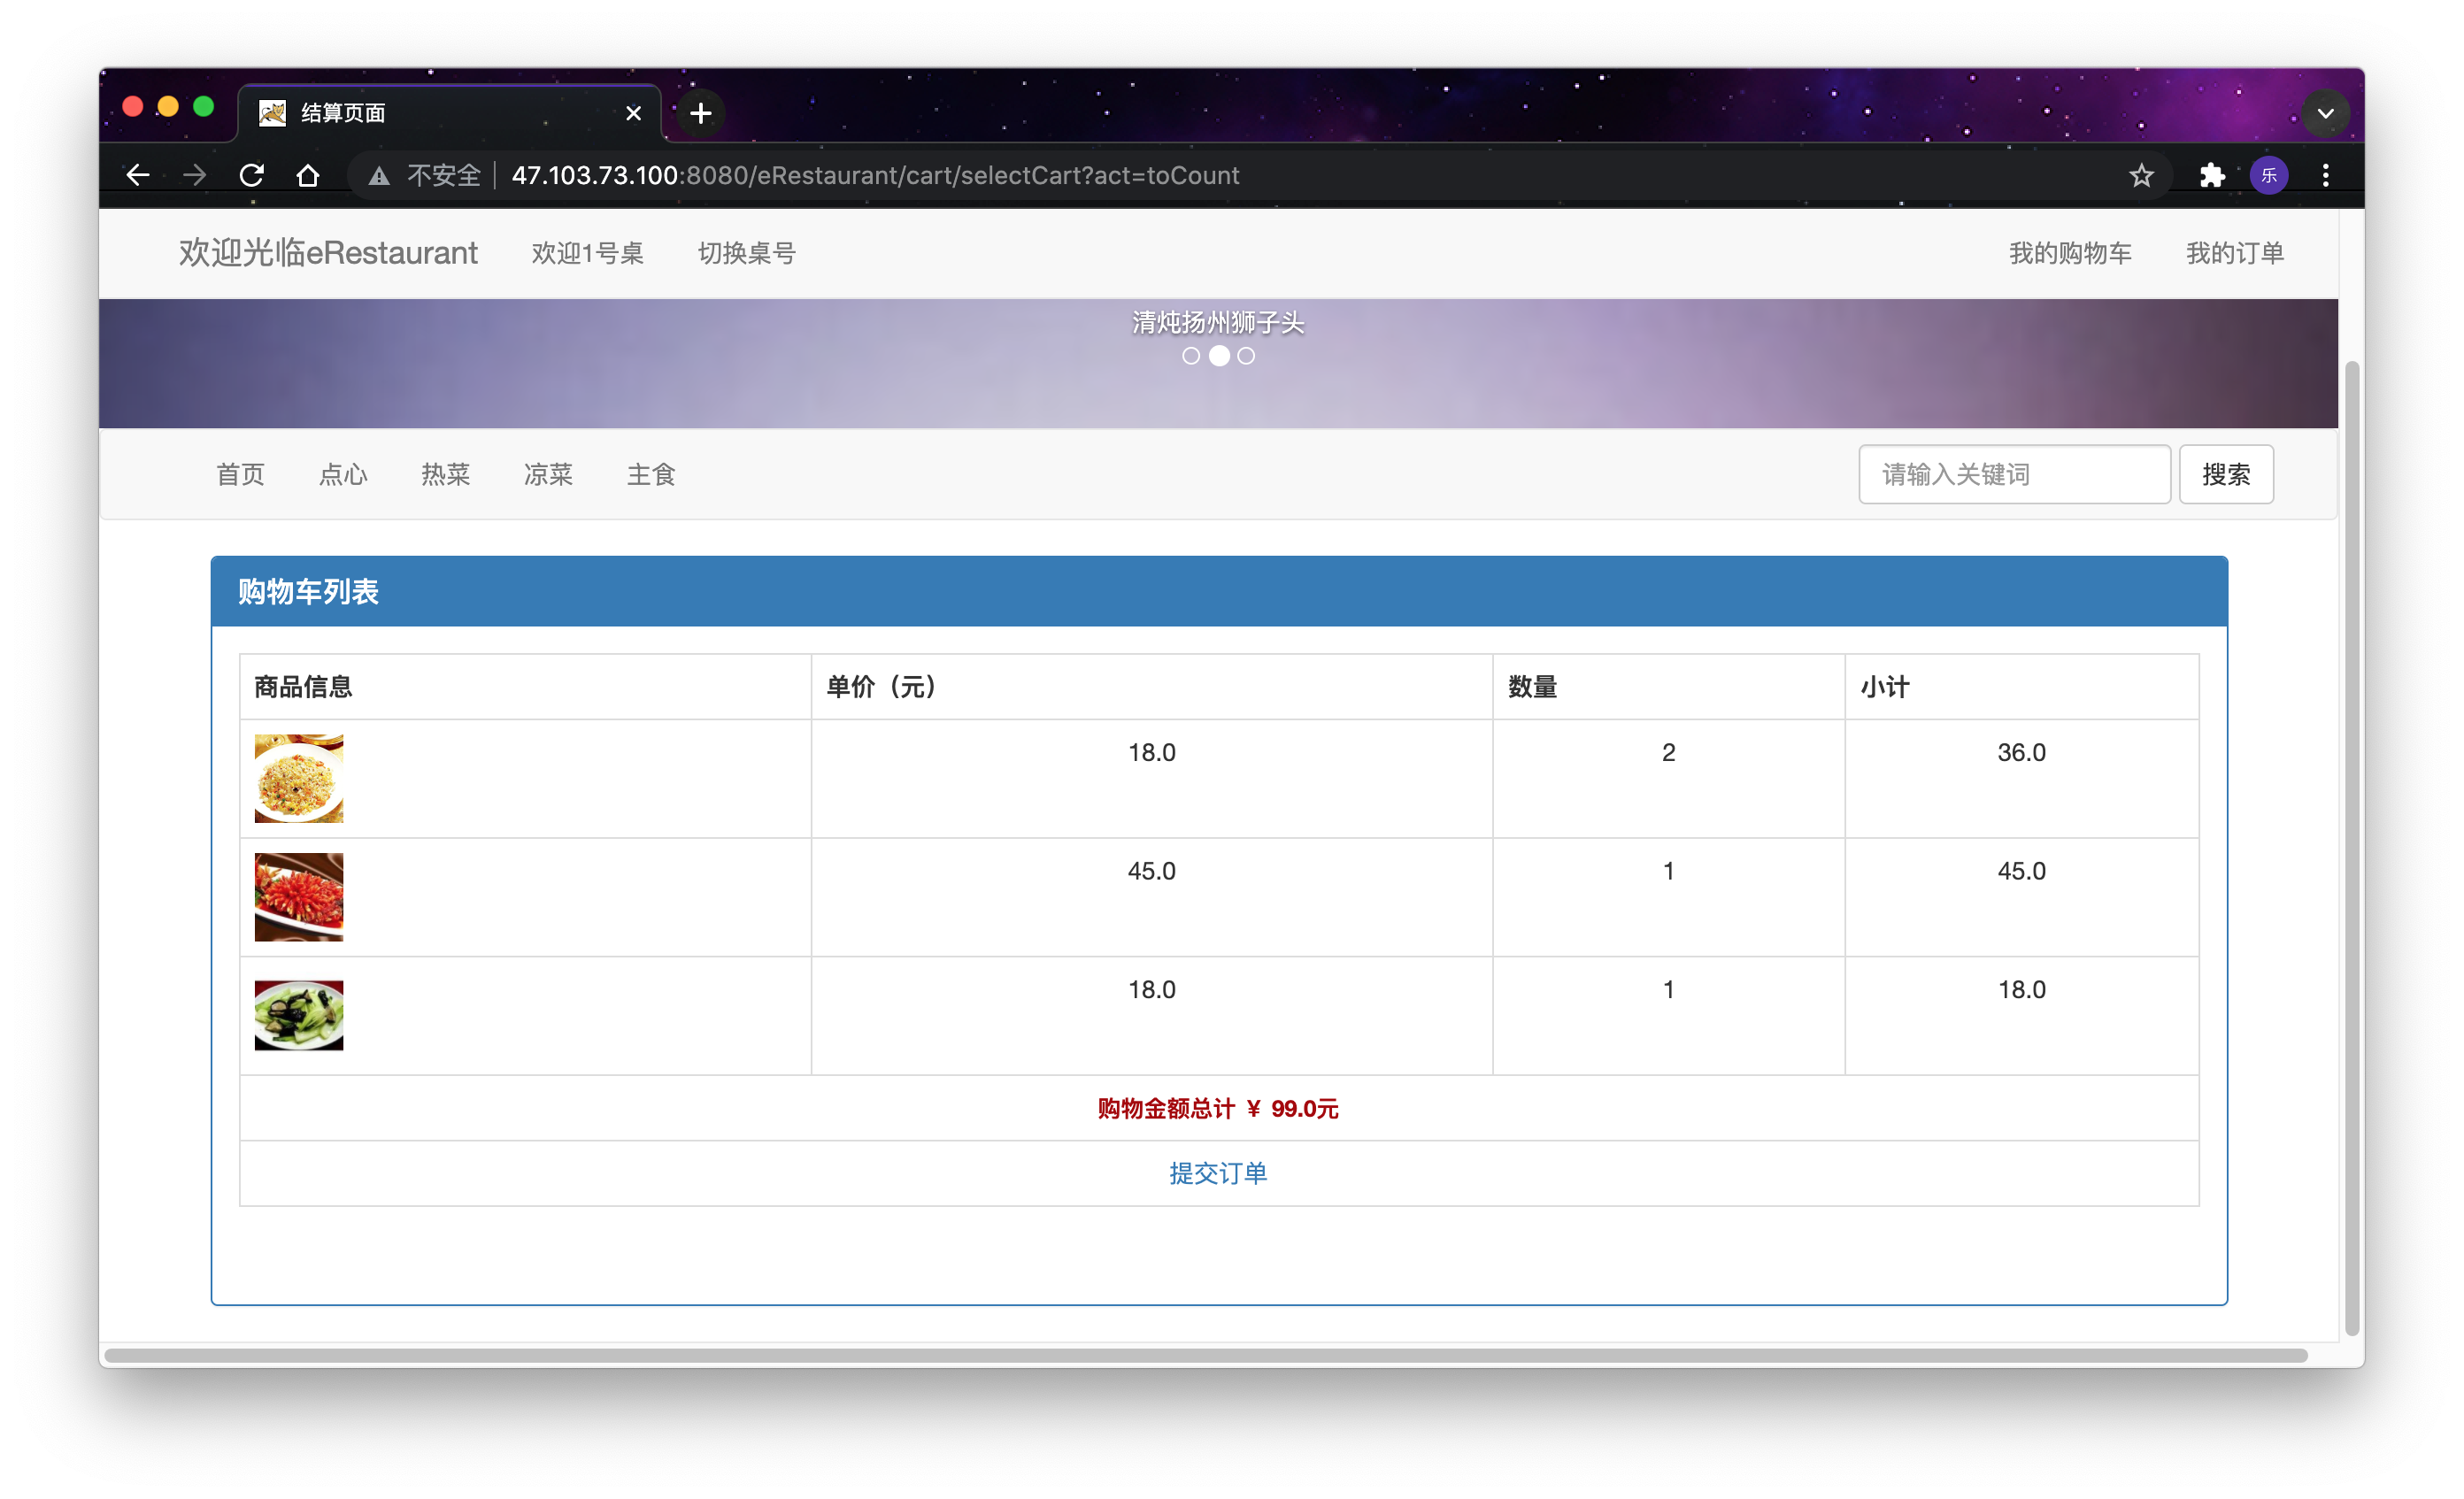
\includegraphics[width=0.8\textwidth]{结算}
      \caption{结算}
      \label{结算}
    \end{figure}

    \begin{figure}[h]
      \centering
      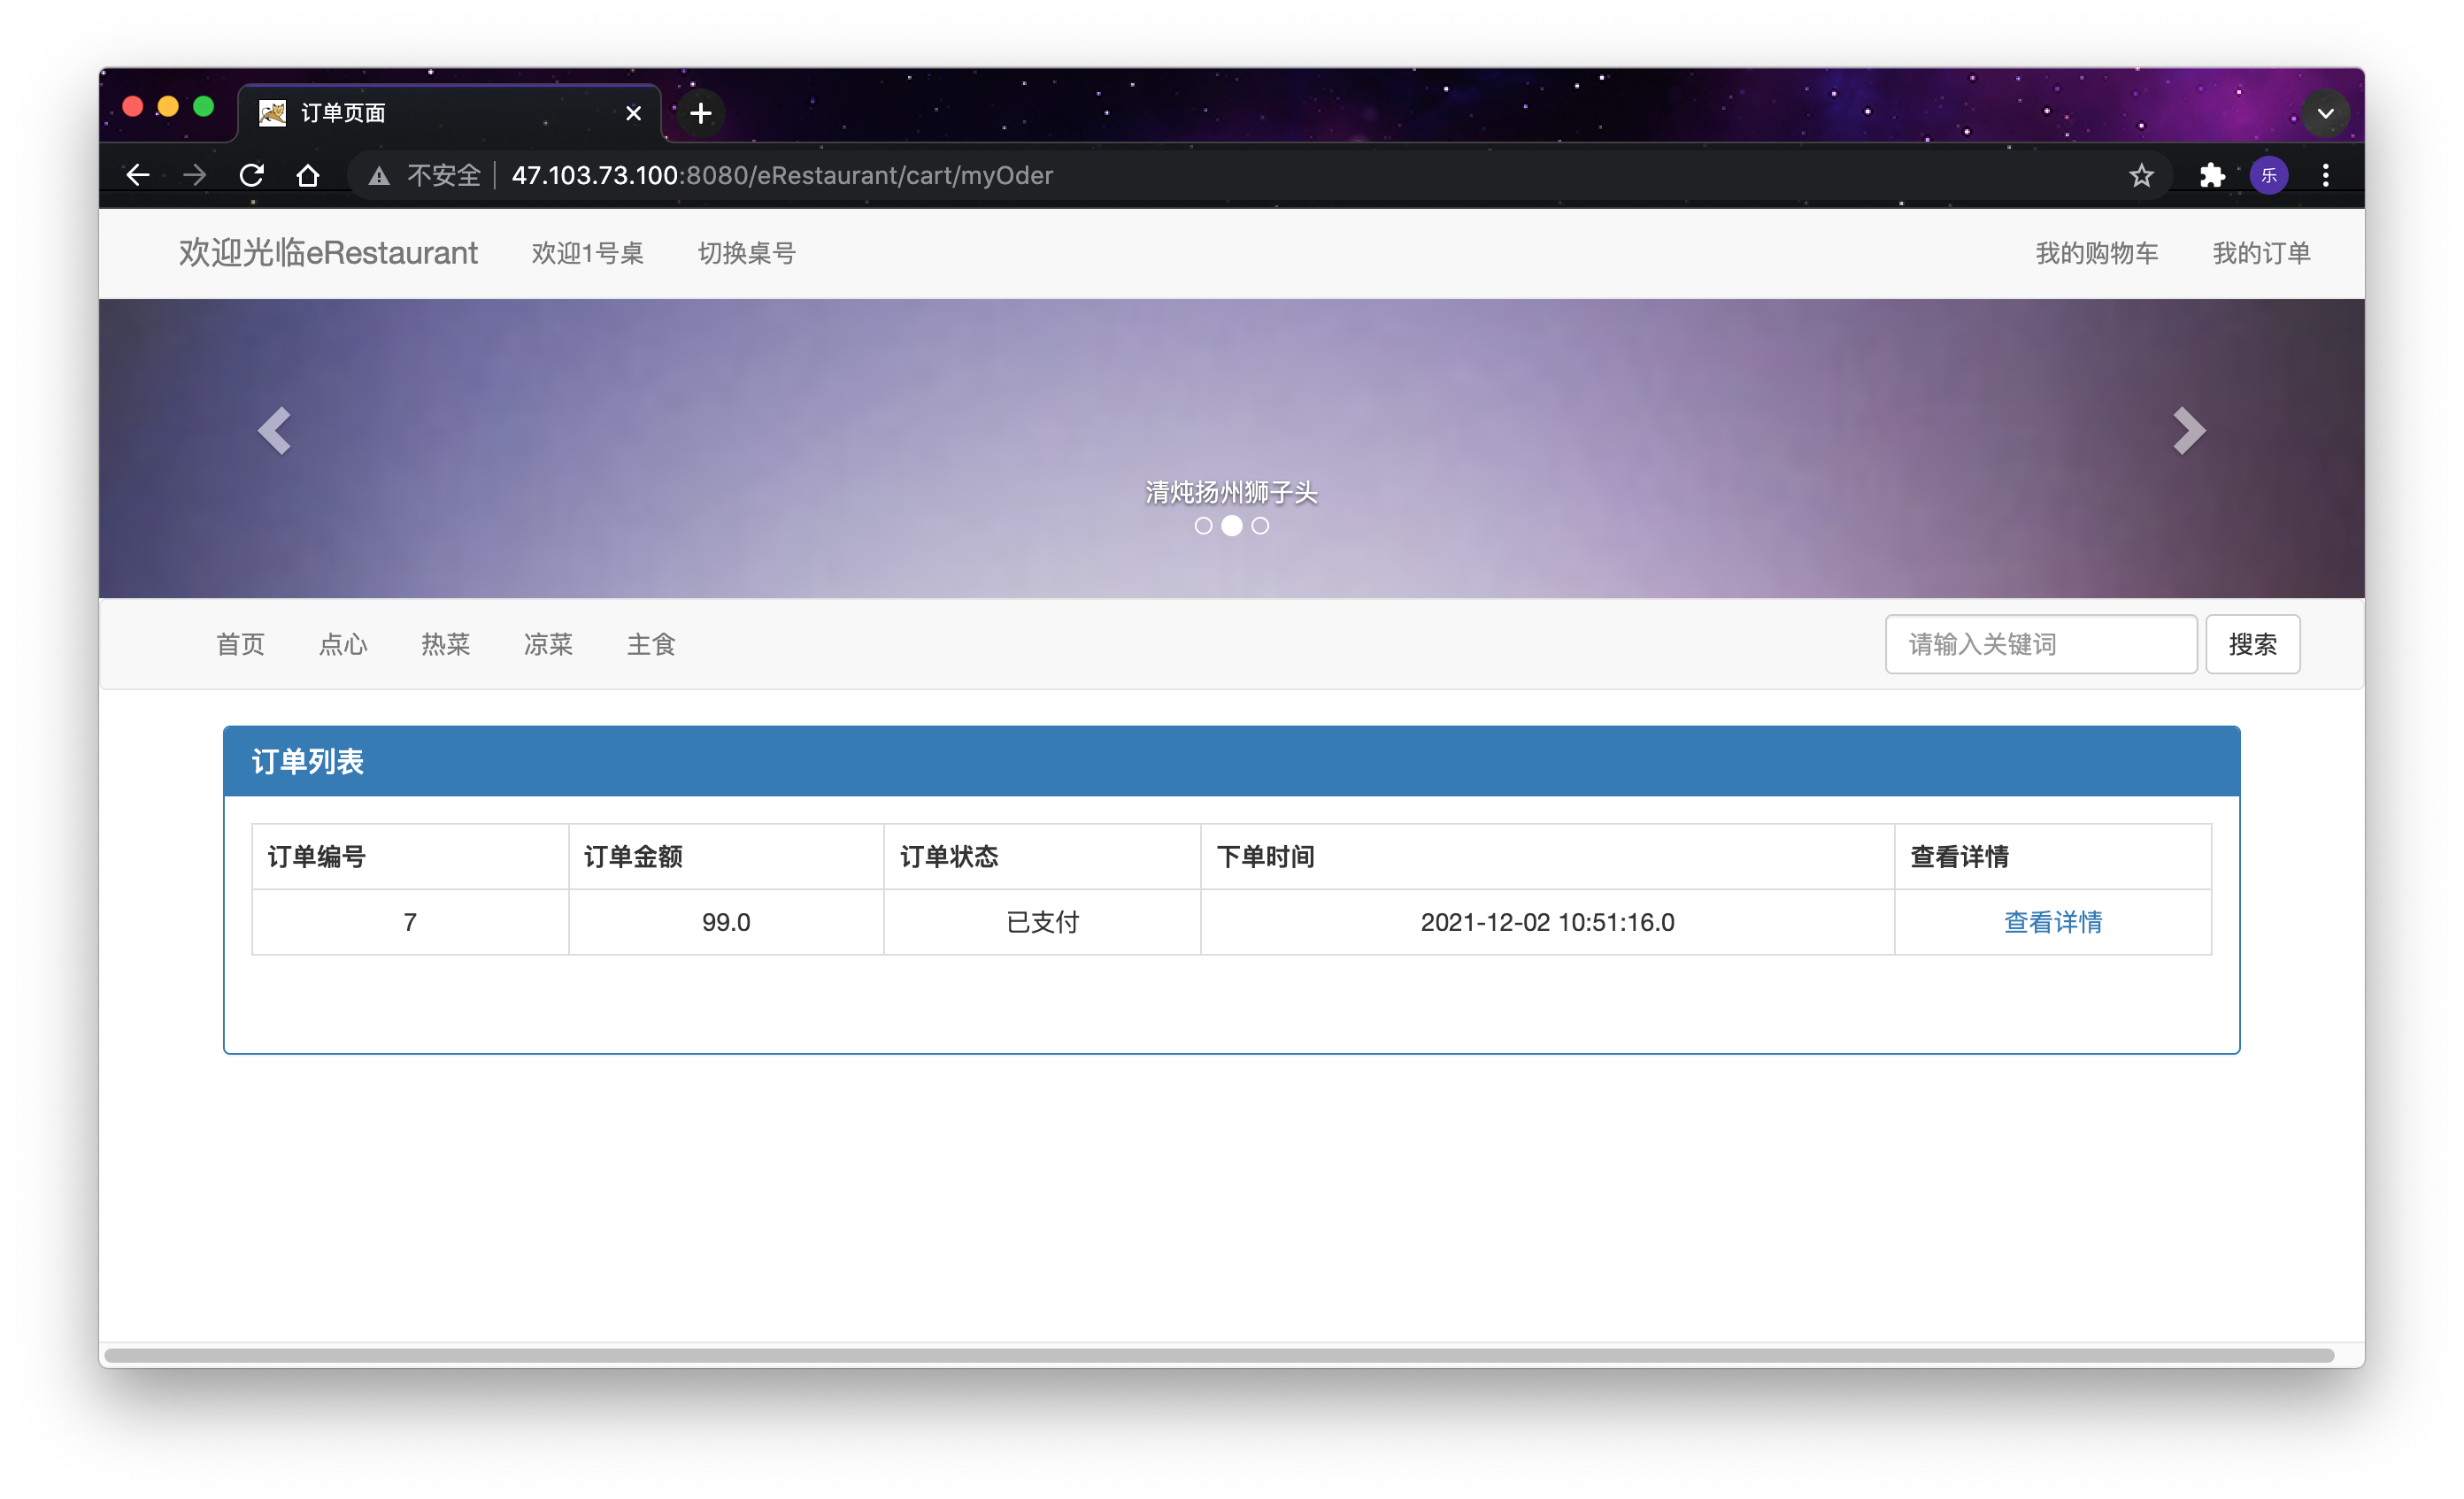
\includegraphics[width=0.8\textwidth]{我的订单}
      \caption{我的订单}
      \label{我的订单}
    \end{figure}

  \subsection*{后台}

  如图\ref{后台登录}-\ref{订单详情}所示。

    \begin{figure}[h]
      \centering
      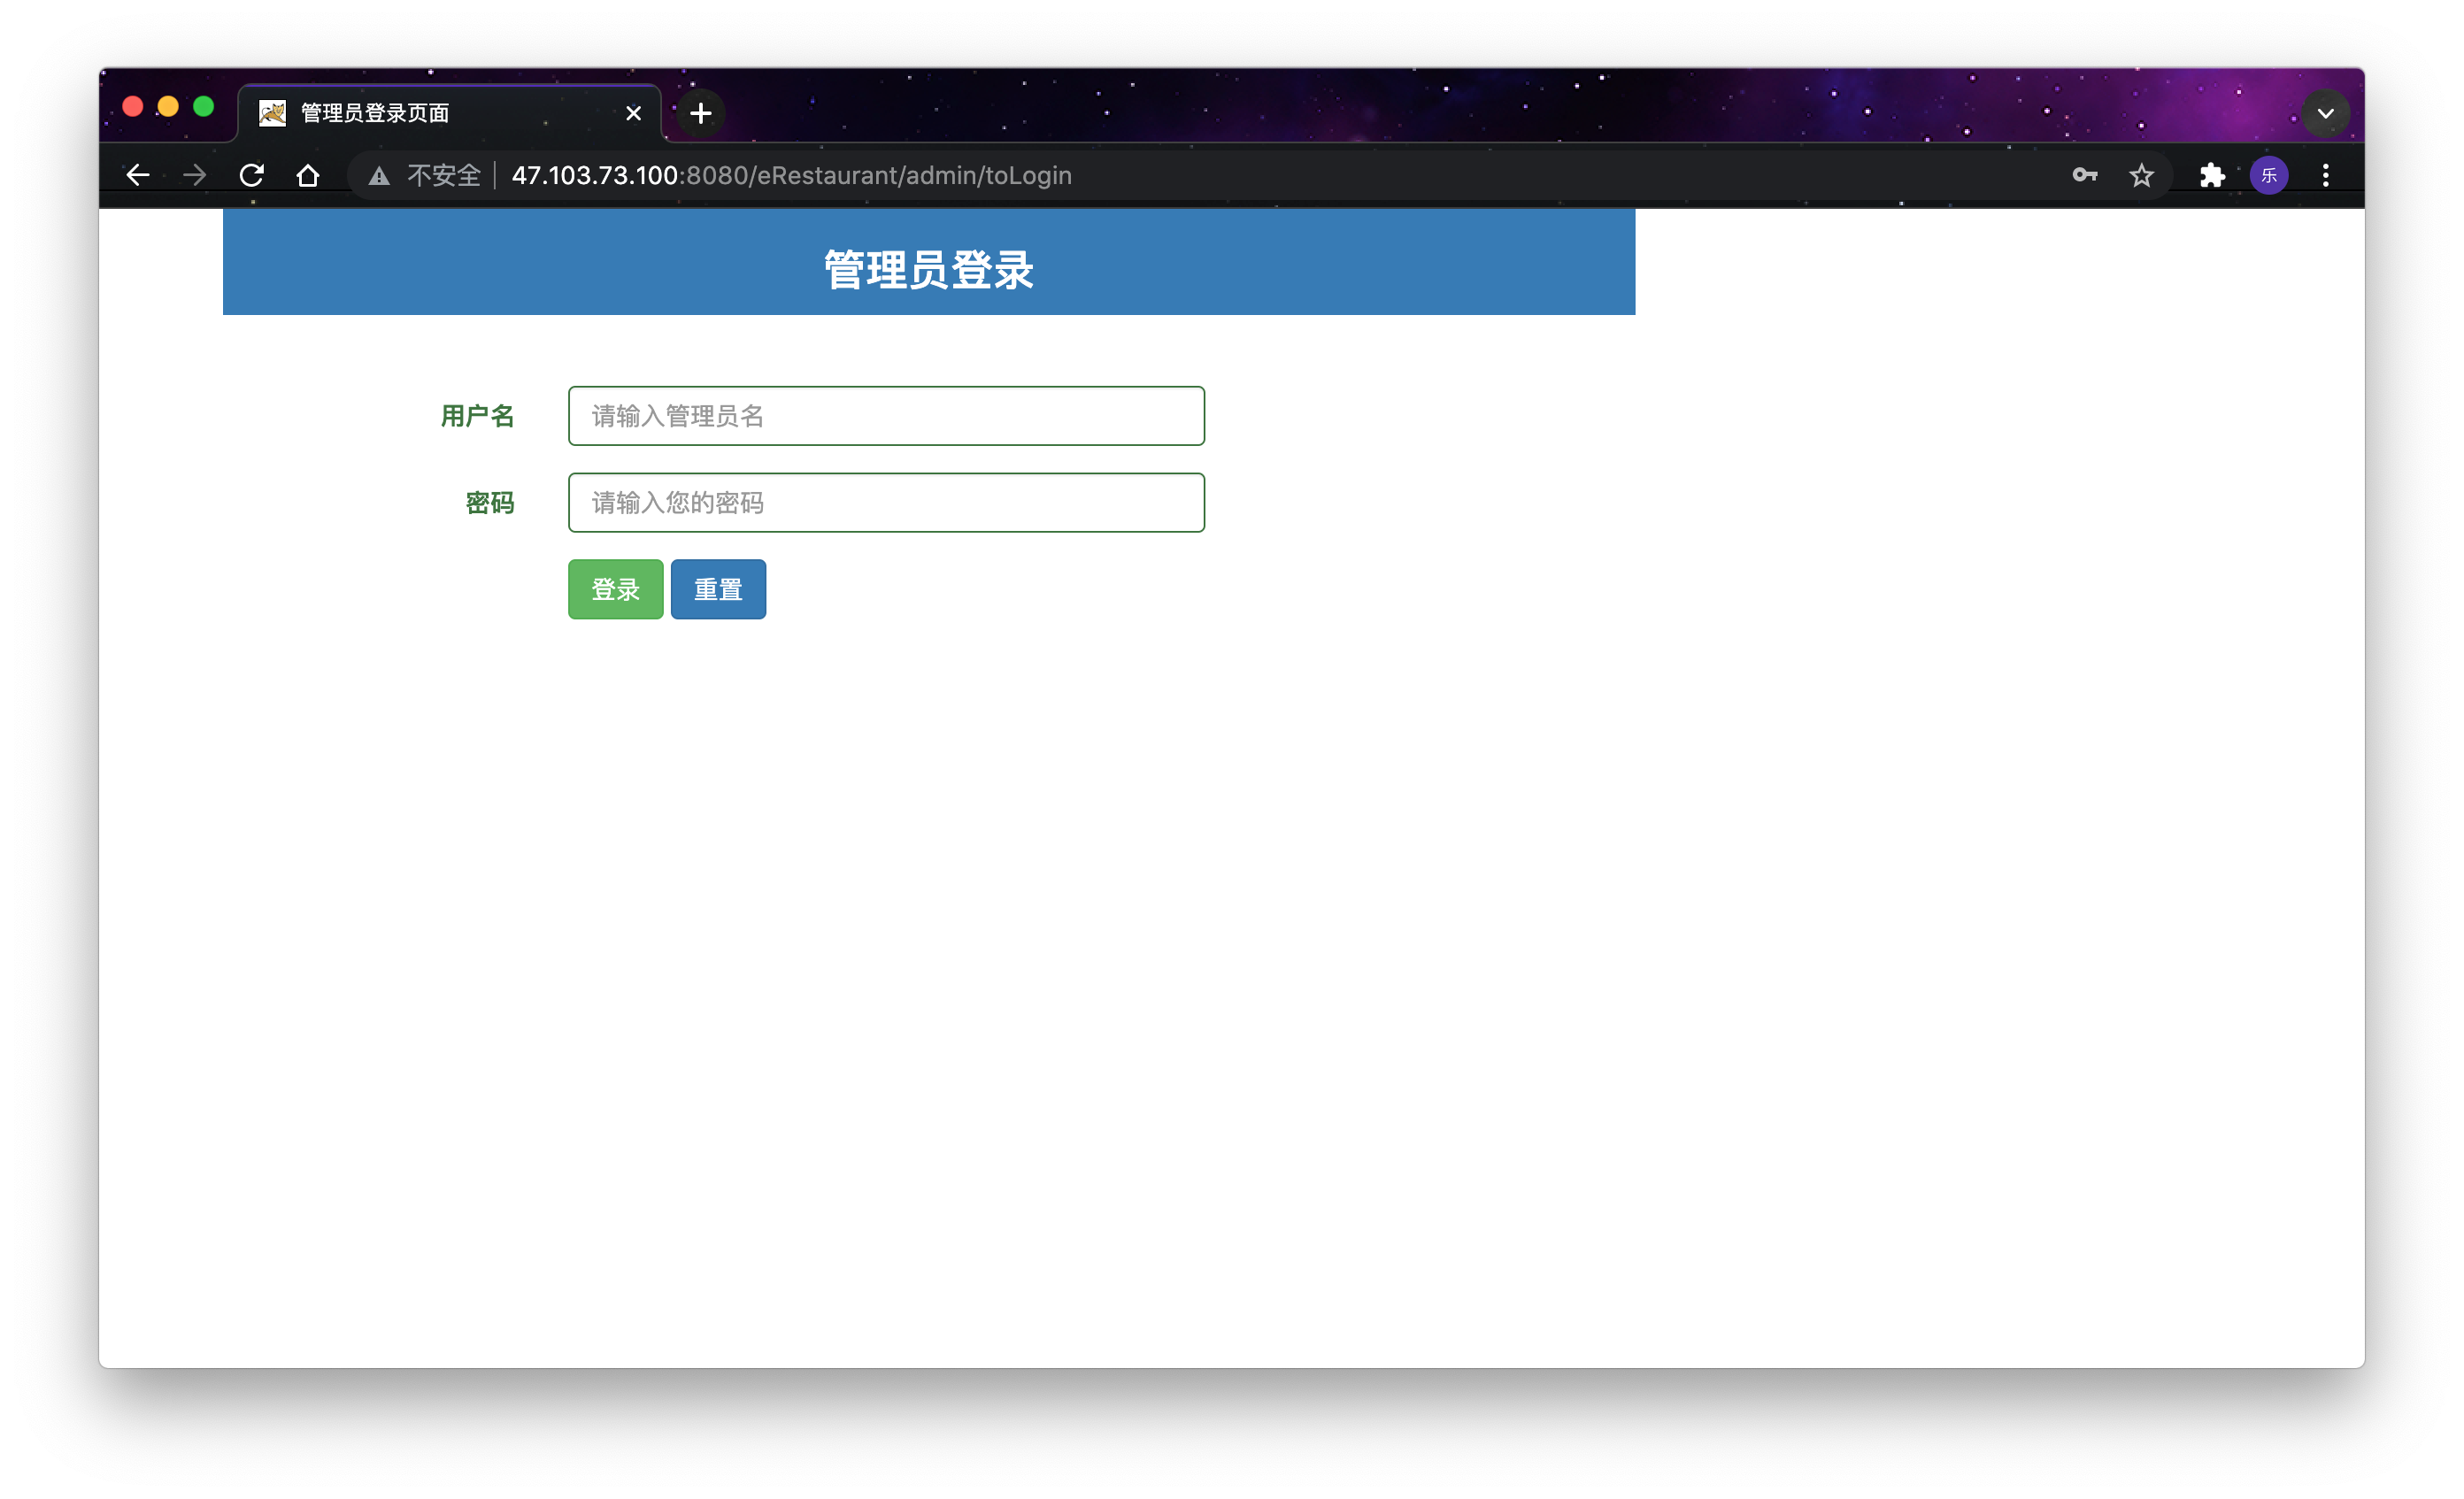
\includegraphics[width=0.8\textwidth]{后台登录}
      \caption{后台登录}
      \label{后台登录}
    \end{figure}

    \begin{figure}[h]
      \centering
      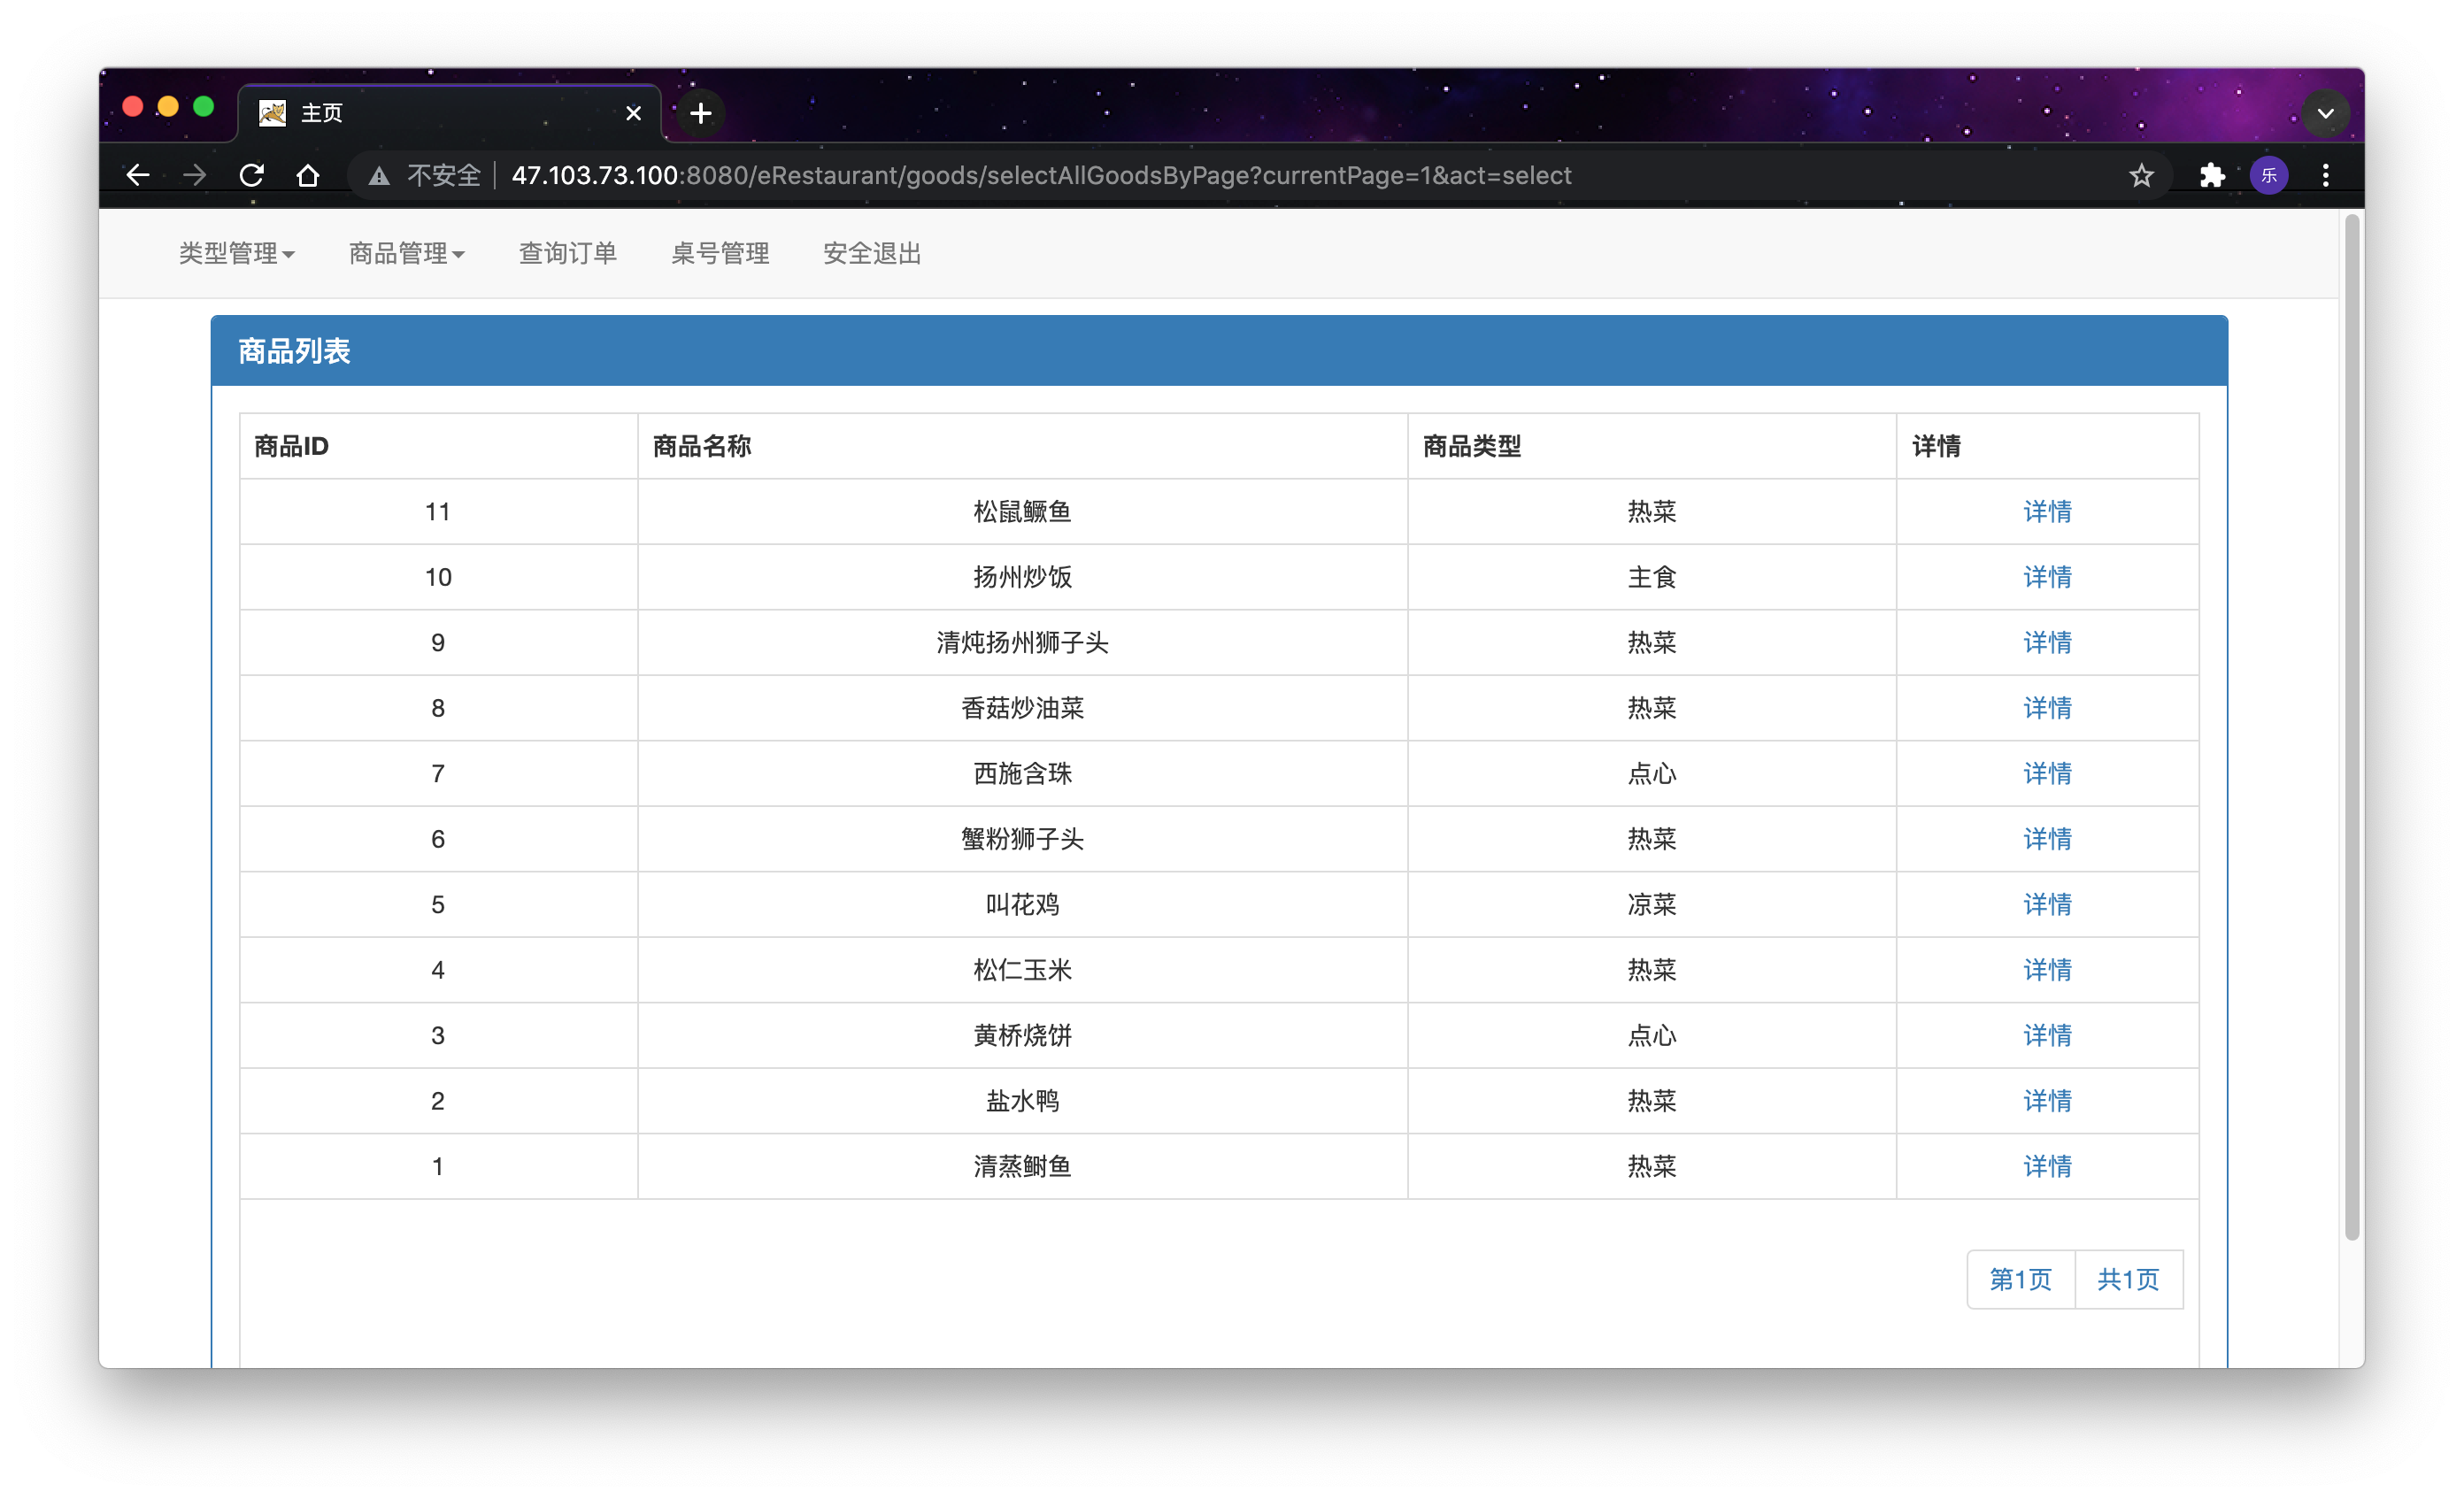
\includegraphics[width=0.8\textwidth]{商品管理}
      \caption{商品管理}
      \label{商品管理}
    \end{figure}

    \begin{figure}[h]
      \centering
      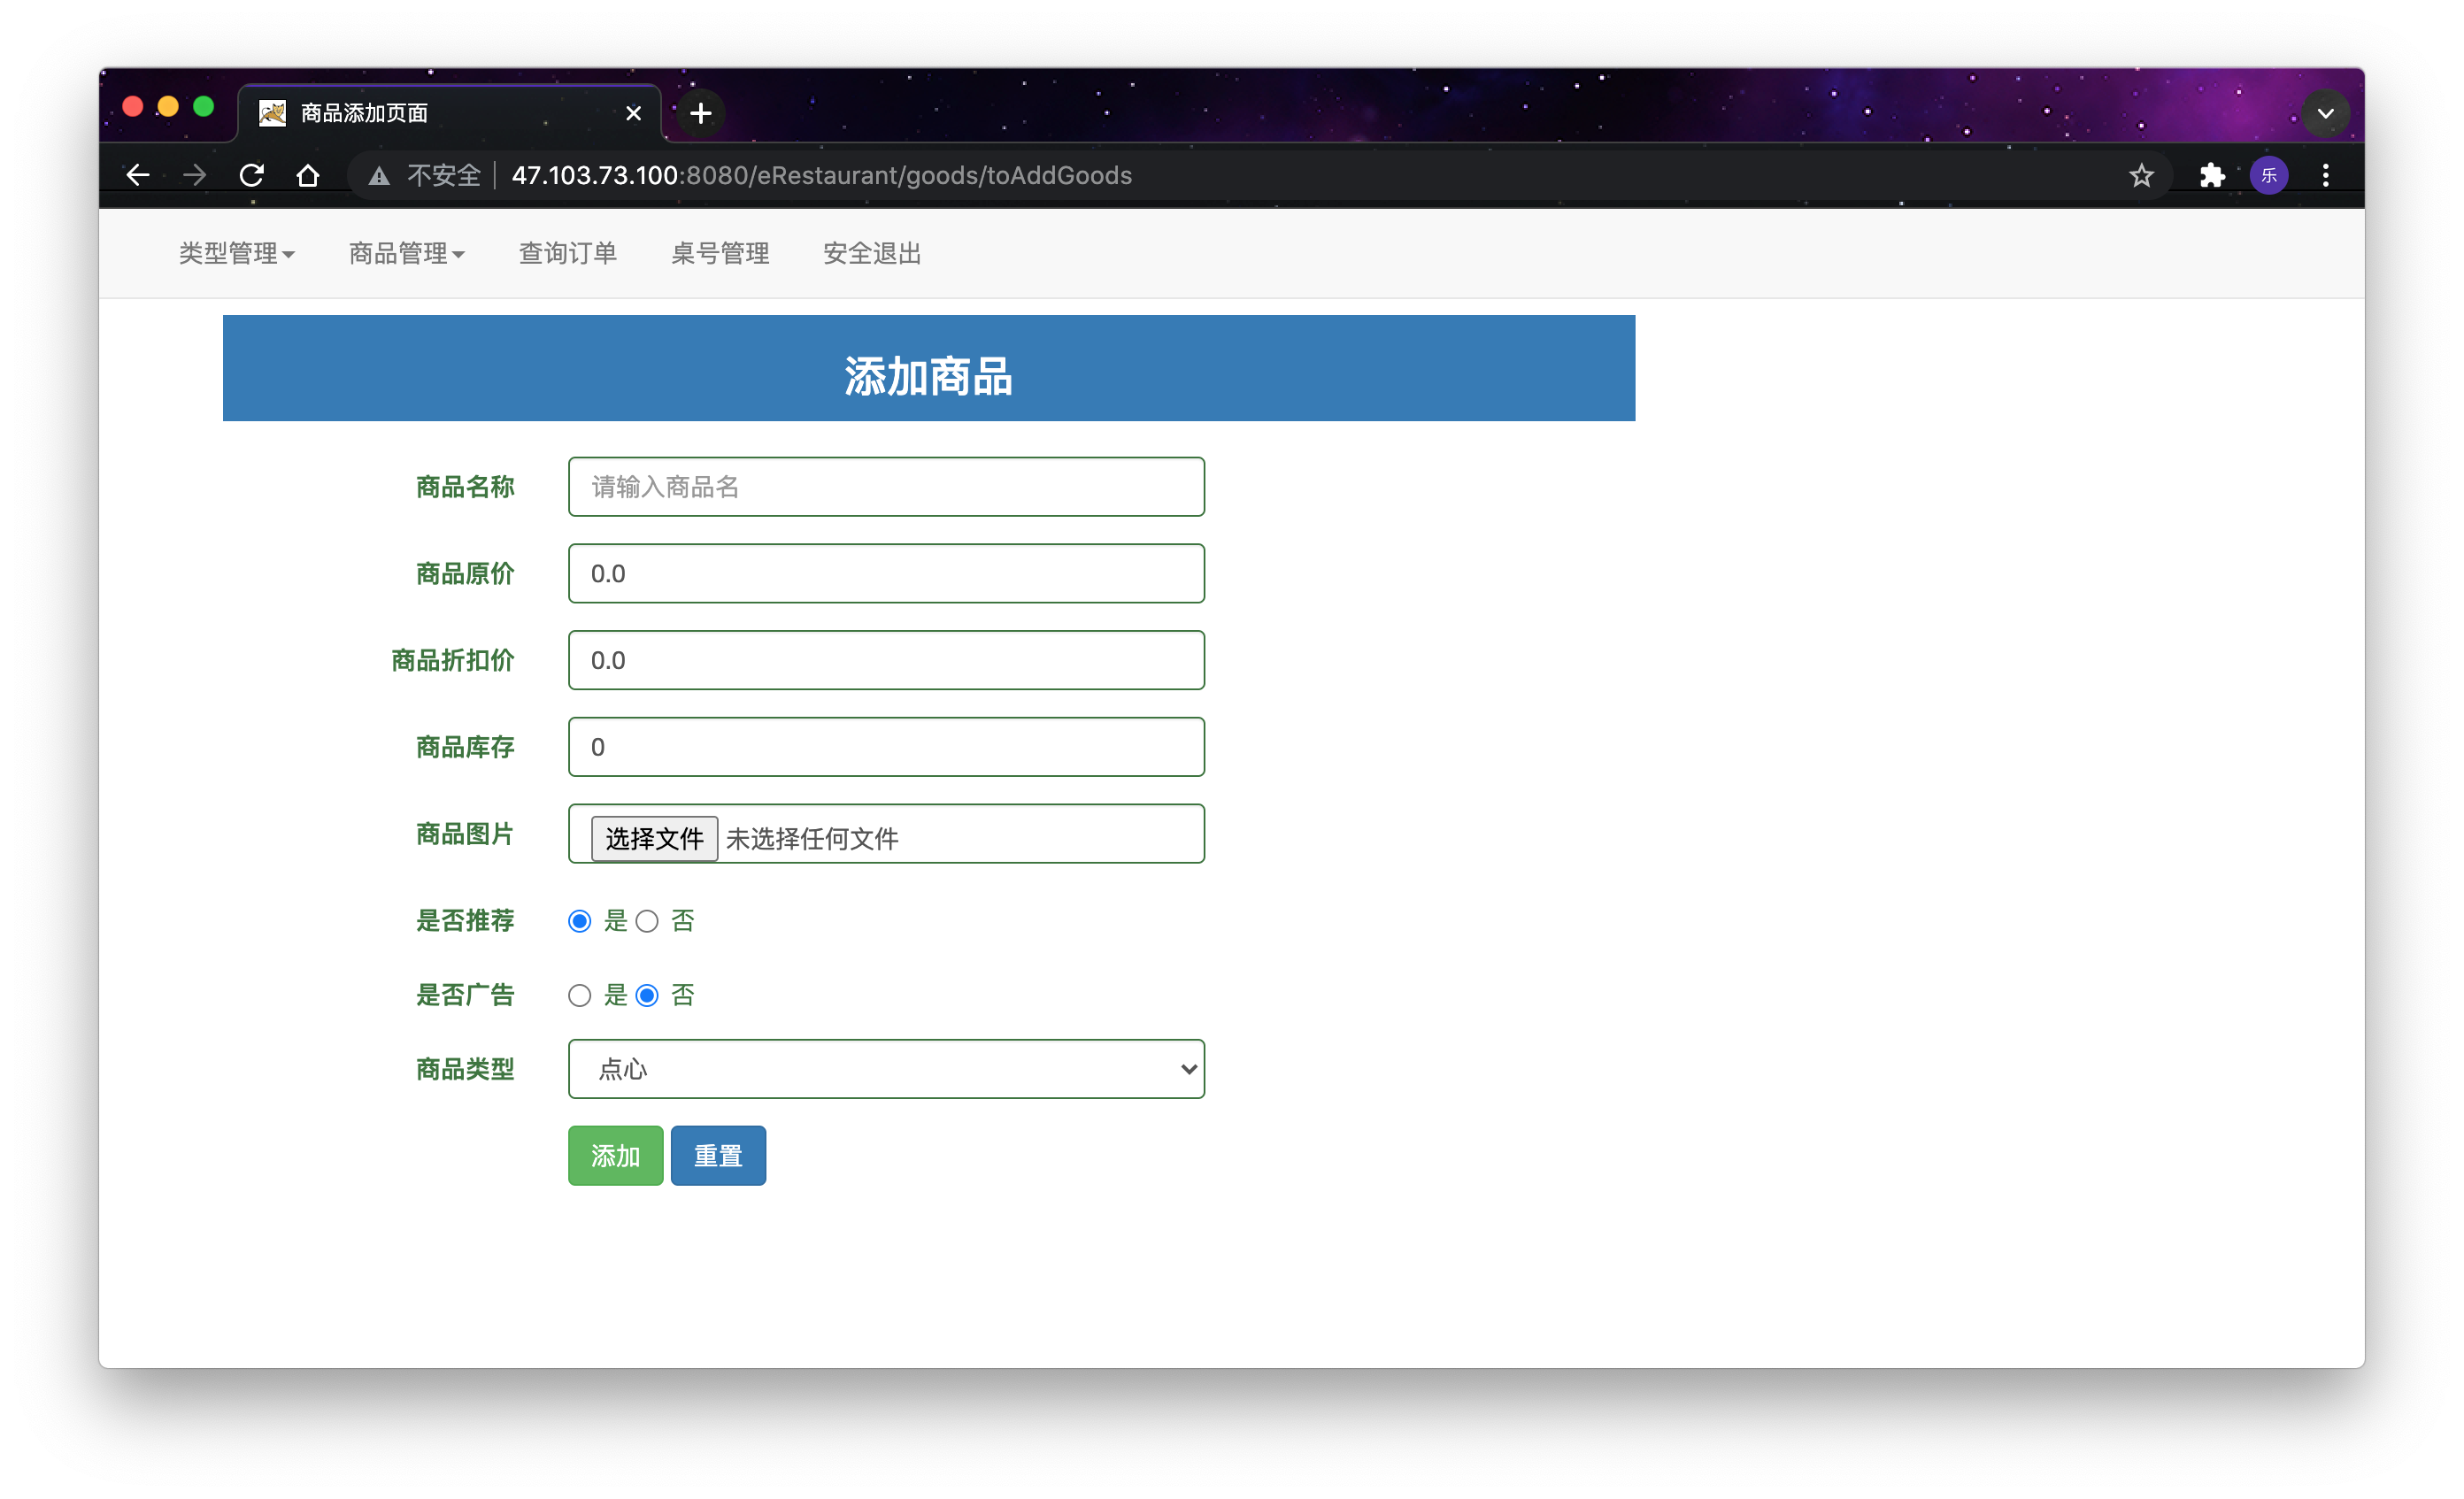
\includegraphics[width=0.8\textwidth]{添加商品}
      \caption{添加商品}
      \label{添加商品}
    \end{figure}

    \begin{figure}[h]
      \centering
      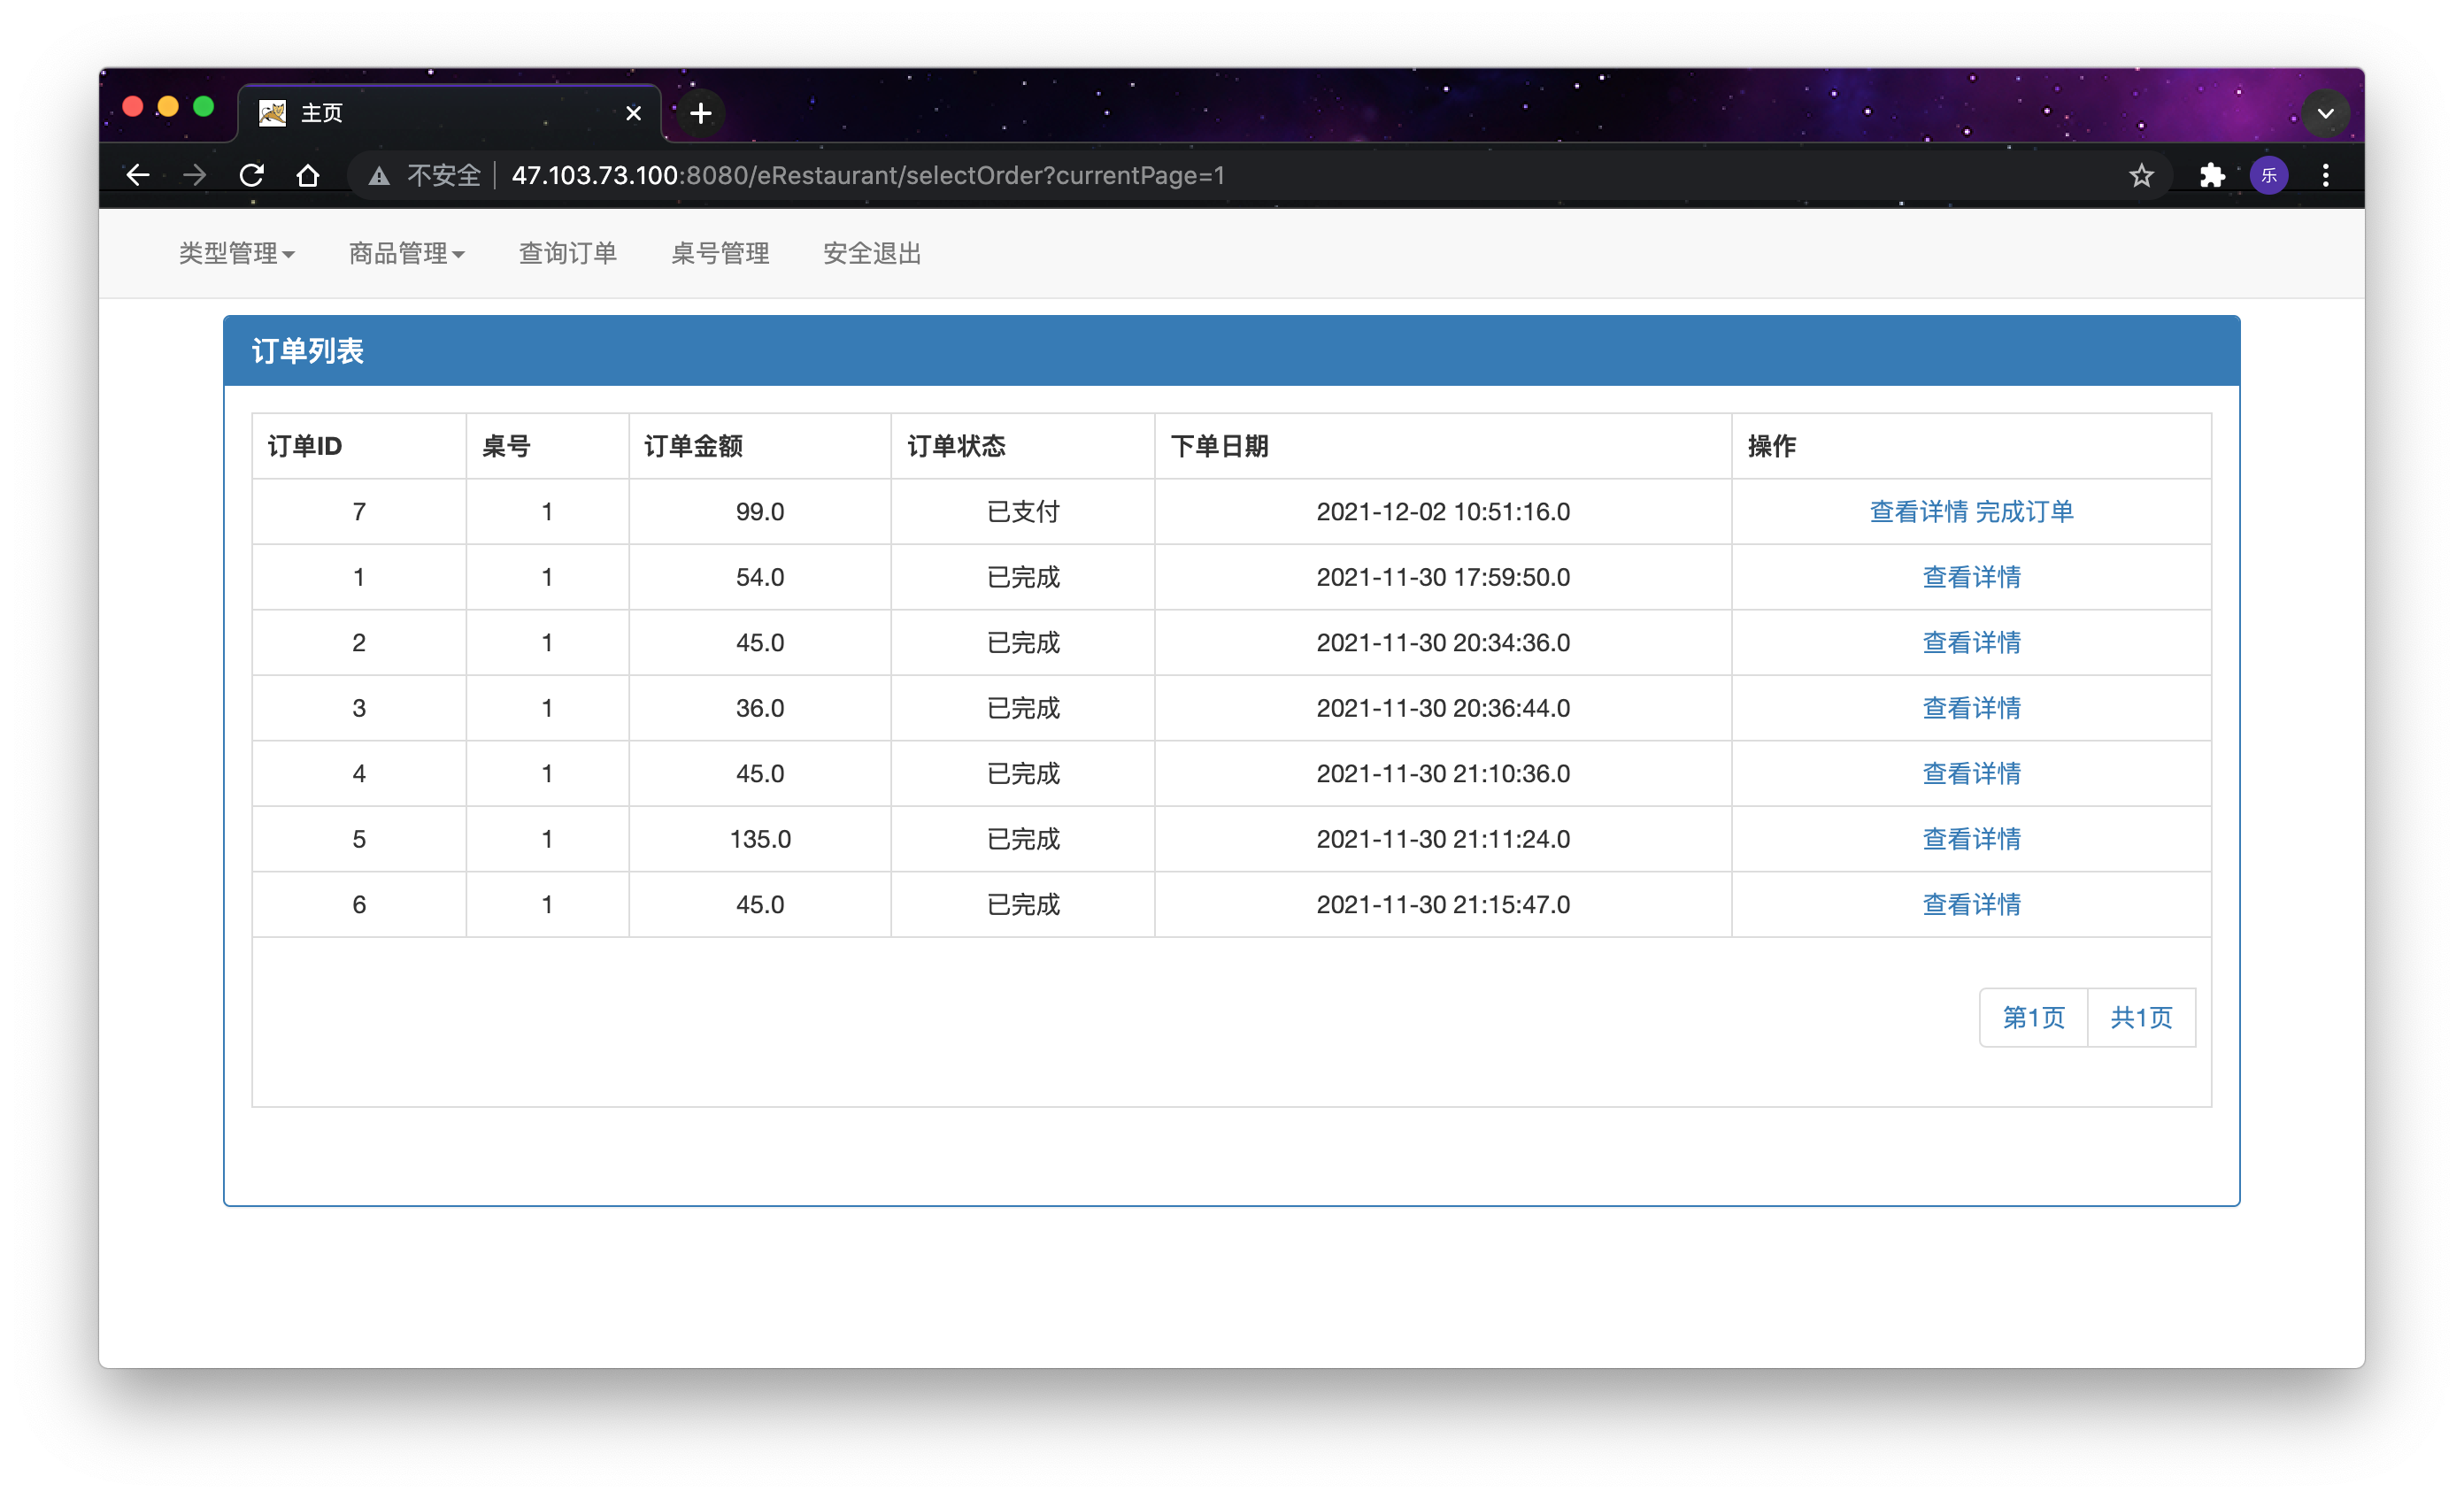
\includegraphics[width=0.8\textwidth]{订单管理}
      \caption{订单管理}
      \label{订单管理}
    \end{figure}

    \begin{figure}[h]
      \centering
      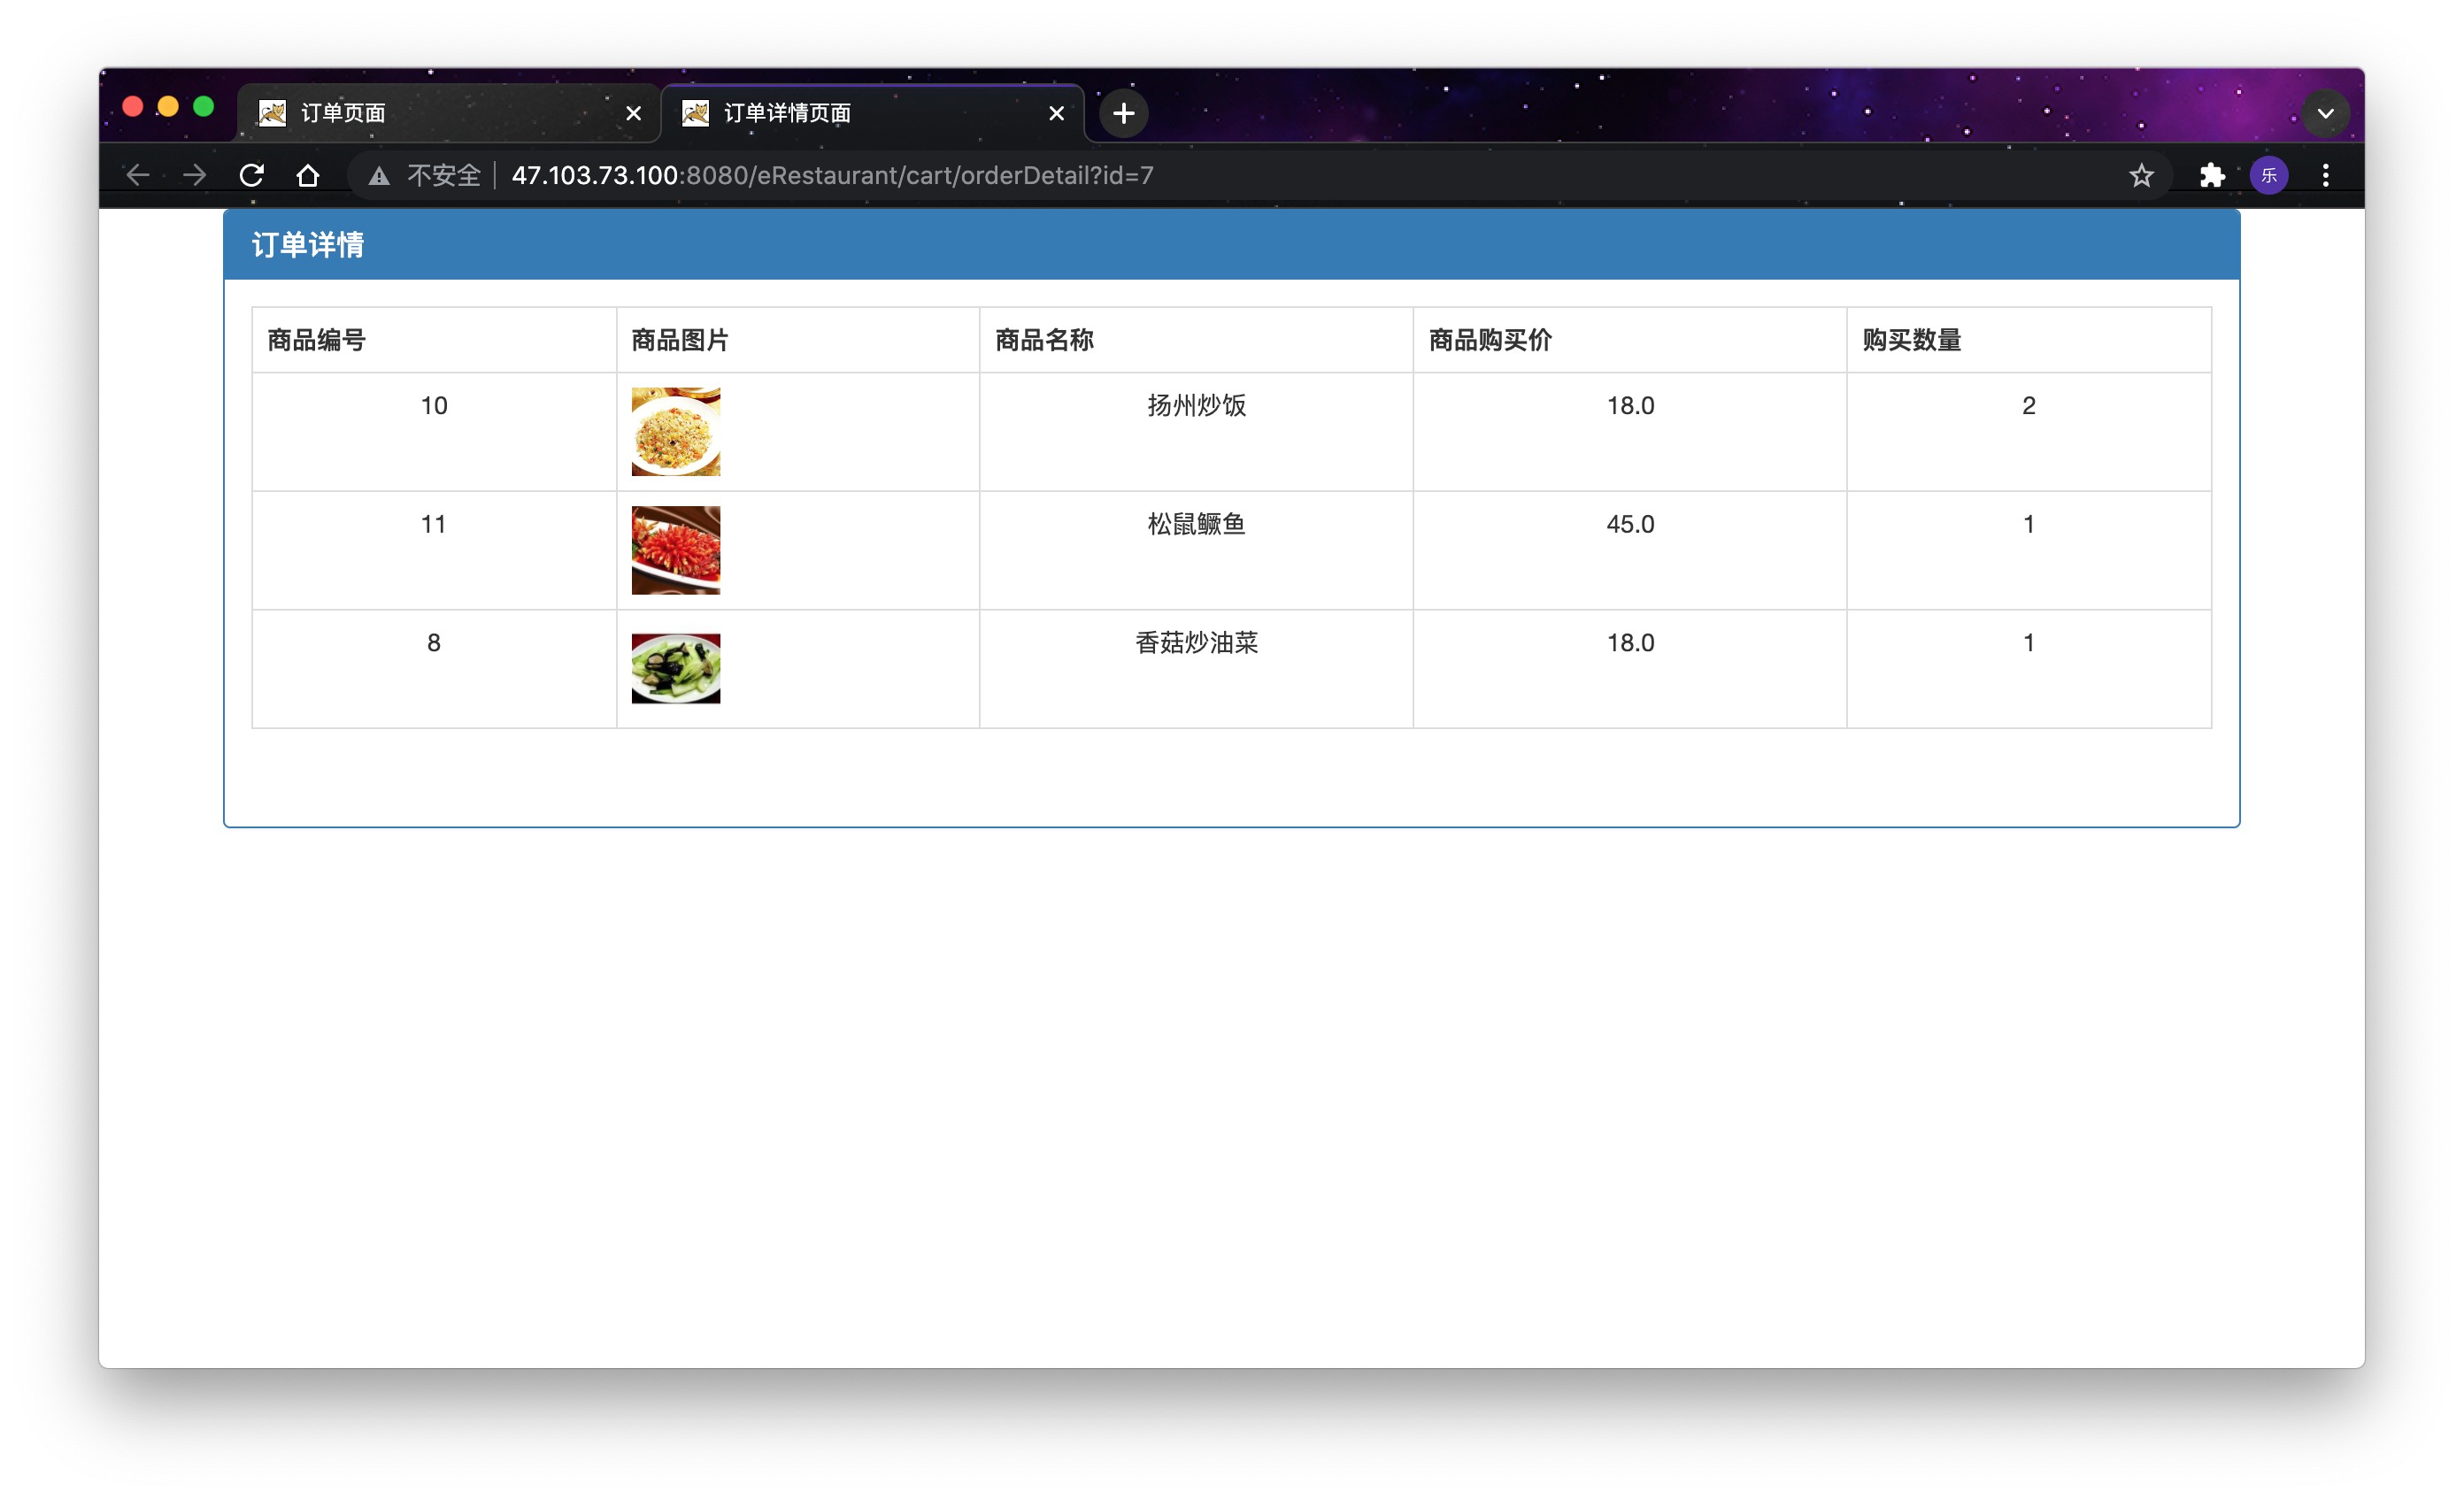
\includegraphics[width=0.8\textwidth]{订单详情}
      \caption{订单详情}
      \label{订单详情}
    \end{figure}

\end{document}